\def\presentationMode{0}
%=========================================================================
%
%  DETERMINE WHAT TO COMPILE
%
%-------------------------------------------------------------------------


\ifdefined\presentationMode
\ifcase\presentationMode\relax
\documentclass[x11names, handout]{beamer}
\or
\documentclass[x11names, trans]{article}
\usepackage{beamerarticle}
\else
\documentclass[x11names]{beamer}
\fi
\else
\documentclass[x11names]{beamer}
\fi


%=========================================================================
%
%  LOAD PACKAGES
%
%-------------------------------------------------------------------------
%\usepackage[x11names,table]{xcolor}
\definecolor{luis}{RGB}{175,160,225}
\usetheme{Boadilla}      % or try Darmstadt, Madrid, Warsaw, ...
\setbeamercolor{frametitle}{fg=white,bg=luis}


\usepackage{polyglossia}
\setmainlanguage{spanish}

\usepackage{todonotes}
\usepackage{fontspec,xunicode}

\usepackage{tabu, colortbl}
\usepackage{hyperref}
\hypersetup{
	bookmarks=true,         % show bookmarks bar?
	colorlinks=true,       % false: boxed links; true: colored links
	linkcolor=black,          % color of internal links
	citecolor=blue,        % color of links to bibliography
	filecolor=magenta,      % color of file links
	urlcolor=black           % color of external links
}


\usepackage{tikz}
\usetikzlibrary{arrows,shapes,positioning,shadows,trees}
\usepackage{pgfplots}
\pgfplotsset{width=10cm, compat=1.10}
\usepackage{ctable}
\newcolumntype{E}{>{$}l<{$}}
\usepackage{multirow}
%\usepackage{wasysym}
\usepackage{graphicx}
\usepackage{multimedia}

	
\usepackage[%
bibstyle=authoryear,%
citestyle=authoryear-icomp,%
sorting=nyt,%
backend=biber,%
url=false,%
uniquename=false,%
doi=false,%
bibencoding=utf8%
]{biblatex} % to format the bibliography
% bib resources are added in course-info.tex file.

%\usepackage{changepage}
\usepackage{etoolbox}
\newtoggle{HIDDEN}
\togglefalse{HIDDEN}

%#================ NEW MATH OPERATORS======================================
\usepackage{amsmath,amsfonts, amssymb} % tools for typing mathematics
\usepackage{xfrac}
%\usepackage{pstricks}
\DeclareMathOperator{\E}{\mathbb{E}}
\DeclareMathOperator{\dd}{\,d\!}
\DeclareMathOperator{\Var}{Var}
\DeclareMathOperator{\Cov}{Cov}
\DeclareMathOperator{\Corr}{Corr}
\DeclareMathOperator{\Prob}{\mathbb{P}}
\newcommand{\MAT}[1]{\begin{bmatrix} #1 \end{bmatrix}}
\newcommand{\argmin}[1]{\underset{#1}{\operatornamewithlimits{argmin}}}
\newcommand{\argmax}[1]{\underset{#1}{\operatornamewithlimits{argmax}}}
\newcommand{\marginal}[2]{\frac{\partial #1}{\partial #2}}
\newcommand{\notation}[2]{\underset{\scriptsize\color{SteelBlue4!60}\text{#2}}{#1}}
\newcommand{\given}[1]{\,|\,#1}

\newcounter{theexample} \setcounter{theexample}{0}

\AtBeginSection{\frame{\sectionpage}}
\AtBeginSubsection{\frame{\subsectionpage}}
\renewcommand{\sectionname}{Sección}
\renewcommand{\subsectionname}{Subsección}

%=========================================================================
%
%  COMMANDS FOR PRESENTATION MODE
%
%-------------------------------------------------------------------------
\mode<presentation>{
	
	\usefonttheme{professionalfonts}
	\renewcommand*{\thefootnote}{\fnsymbol{footnote}}
	
	\newcommand{\ITEM}[2]{%
		\begin{tabu} to \textwidth {>{\color{white}\columncolor{DodgerBlue4}}X[1,c,m]>{\small}X[4,l,m]}
			#1 & #2 \\
		\end{tabu}
	}
	
	\newcommand{\EQ}[2]{%
		\begin{tabu} to \textwidth {>{\color{white}\columncolor{teal}\scriptsize}X[1,c,m]>{\columncolor{orange!10}\small}X[4,c,m]}
			\textbf{#1} & \begin{equation*}   #2 \end{equation*}\\
		\end{tabu}
	}

	\newcommand{\CONCEPT}[4]{%
        \extrarowsep =0.75em
		\begin{tabu} to #1\textwidth {>{\color{white}\columncolor{teal}\scriptsize}X[1,c,m]>{\columncolor{teal!15}\small}X[#2,p,m]}
			\textbf{#3} &  #4 \\
		\end{tabu}
	}	

	\newenvironment{EXAMPLE}[1]{%
		\stepcounter{theexample}
		\setbeamercolor{background canvas}{bg=purple!25}
		\begin{frame}[plain,noframenumbering]
			\LARGE Ejemplo \arabic{theexample}:
			
			\huge #1
		\end{frame}
		\setbeamercolor{background canvas}{bg=purple!12}
		}{
		}

	\newenvironment{SIDENOTE}[1]{%
		\setbeamercolor{background canvas}{bg=orange!8}
		\begin{frame}{Side note: #1}
	}{
		\end{frame}
	}

}



%=========================================================================
%
%  COMMANDS FOR ARTICLE MODE
%
%-------------------------------------------------------------------------
\mode<article>{
	\usepackage[top=1in, bottom=1.25in, left=1.25in, right=1.25in]{geometry}
	
	\newcommand{\ITEM}[2]{%
		\begin{tabu} to \textwidth {X[1,c,m]X[4,l,m]}
			\hline
			#1 & #2 \\ \hline
		\end{tabu}
	}
	
	\newcommand{\EQ}[2]{%
		\begin{tabu} to \columnwidth {X[1,cm]X[4,lm]}
			\rowcolor{orange!10}
			#1 & \begin{equation*}   #2 \end{equation*}\\ 
		\end{tabu}
	}

	\usepackage{framed}
	\newenvironment{EXAMPLE}[1]{%
		\stepcounter{theexample}
		\begin{framed}
			\colorbox{teal}{\textcolor{white}{\Large Ejemplo
            \arabic{theexample}: #1}} 
			\vspace{1em}		\\
	}{
		\end{framed}
	}
	
	\newenvironment{SIDENOTE}[1]{%
	\begin{framed}
		\colorbox{orange!80!black}{\textcolor{white}{Side note: #1}} 
		}{
	\end{framed}
}

}



%=========================================================================
%
%  COMMANDS FOR ALL MODES
%
%-------------------------------------------------------------------------
    \makeatletter
    \patchcmd{\beamer@sectionintoc}{\vskip1.5em}{\vskip0.5em}{}{}
    \makeatother

\newcommand{\makeFrameTitle}{%
	\begin{frame}[plain,noframenumbering]%
	\begin{textblock*}
		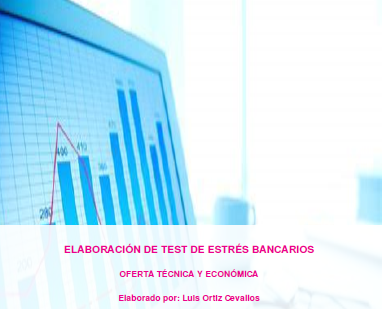
\includegraphics[height=2.0cm]{imag/LUIS.png}\hfill\includegraphics[height=2.0cm]{imag/atlantida.png}
	\end{textblock*}
	\vspace{0.5cm}\maketitle%
	\end{frame}%
	
		
	\begin{frame}[plain,noframenumbering]{Contenido}    
		\setbeamertemplate{section in toc}[sections numbered]
		\setbeamertemplate{subsection in toc}[subsections numbered]	
		\tableofcontents
	\end{frame}
	
}

\newcommand{\contn}{\hfill(cont'n)}



\newcommand{\makeReferencesFrame}[1]{
	\begin{frame}[fragile,allowframebreaks]
		\nocite{#1}
		\printbibliography
	\end{frame}
}


\newcommand{\CASE}[1]{ \colorbox{Coral4}{\color{white} #1} \vspace{1em}}


\newcommand{\IMPORTANT}[1]{%
	\begin{tabu}  {>{\columncolor{DodgerBlue4!10}}X[c,m]}
		\begin{equation*} #1 \end{equation*}\\
	\end{tabu}
}


\newcommand{\NOTICE}[1]{%
	\begin{tabu} {>{\columncolor{Yellow1!30}}X[c,m]}
		\begin{equation*} #1 \end{equation*}\\
	\end{tabu}
}



\newcommand{\colorblock}[3]
{\begingroup
	\setbeamercolor{block title}{bg=#1,fg=white}
	\setbeamercolor{block body}{bg=#1!6}
	\begin{block}{#2}
		#3
	\end{block}
	\endgroup
}


%-------------------------------------------------------------------------

\newcommand{\rojitas}[1]{\textbf{{\color{red} #1}}} 
\newcommand{\negritas}[1]{\textbf{#1}} 
\newcommand{\espacio}{\vspace{1em}}
\newcommand{\itemdos}{\item[\checkmark]}
\newcommand{\flechas}{\item[$\rightarrow$]}


\newcommand{\ALTERNATE}[2]{%
	\only<article>{#1}\only<presentation>{#2}
}





\usepackage{pgfpages}
\pgfpagesuselayout{2 on 1}[letterpaper,border shrink=5mm]


\author[Luis Ortiz Cevallos e-mail: \href{leortiz@uc.cl}{\textit{leortiz@uc.cl}}]{Profesor: Luis Ortiz Cevallos, e-mail:\href{leortiz@uc.cl}{\textit{leortiz@uc.cl}} }
\title[MICROECONOMÍA DE LA BANCA]{\vspace*{1.0em} MICROECONOMÍA DE LA BANCA}
\date[\href{https://ortiz-cevallos.github.io/luisortiz.github.io/ }{\textit{https://ortiz-cevallos.github.io/luisortiz.github.io/}}]{}



\addbibresource{econometria-referencias.bib}






%\includeonly{02-Conceptos-basicos}






\begin{document}
\makeFrameTitle

\section{Aversión y premio por riesgo}
\begin{frame}
\frametitle{Aversión al riesgo y premio de riesgo}

Un individuo se dice que es averso al riesgo si y sólo si:
\\

\textit{Su función de utilidad es concova, implicando que este sujeto no aceptaría participar en un ``juego justo'' (fair lottery).\\
     Un ``juego justo'' es definido como aquel cuyo valor esperado es cero.}\\

Un ejemplo:\\
Supongamos un ``juego justo'' que tiene un pago aleatoria de $ \hat{\epsilon}$, donde:

\[
\hat{\epsilon}= \left\{ \begin{array}{lcl}
h_{1} & con\; probabilidad & p \\
& & \\
h_{2} & con\; probabilidad & 1-p
\end{array}
\right.
\] 

Por tanto para ser un ``juego justo'' debe cumplirse:
\begin{align}
E(\hat{\epsilon})&=ph_{1}+(1-p)h_{2}=0 \nonumber \\
ph_{1}&=-(1-p)h_{2} \nonumber \\
\frac{h_{1}}{h_{2}}&=-\frac{(1-p)}{p}\nonumber
\end{align}    
\end{frame}


\begin{frame}
    \frametitle{Aversión al riesgo y premio de riesgo}
  Es de notar que si el individuo acepta el ``juego justo'', considerando una función de utilidad esperada a VNM tendría:
\begin{align}
V&=E(U(W+\hat{\epsilon}))\nonumber 
\end{align}    
 Mientras si no acepta participar en el juego justo tendría:
 \begin{align}
 V&=E(U(W))=U(W)\nonumber 
 \end{align}     

Por tanto un individuo es averso al riesgo si se cumple:
\begin{align}
U(W)&> E(U(W+\hat{\epsilon}))=pU(W+h_{1})+(1-p)U(W+h_{2})\nonumber 
\end{align}  
  
\end{frame}


\begin{frame}
    \frametitle{Aversión al riesgo y premio de riesgo}
   Es posible definir el grado de aversión al riesgo de un individuo, para ello definimos el concepto ``premio por riesgo'' que significa la cantidad de un bien que el sujeto está dispuesto a pagar para evitar el riesgo.\\
   Definiendo $\pi$ como el ``premio por riesgo'' de un individuo dado un ``juego justo'' $\hat{\epsilon}$ de manera que el valor máximo que el individuo estaría dispuesto a pagar para evitar el riesgo estaría dado por:
   \begin{align}
   U(W-\pi)&= E(U(W+\hat{\epsilon}))
   \end{align}  
   
    
\end{frame}

\begin{frame}
\frametitle{Aversión al riesgo y premio de riesgo}
Ahora bien, que sucede si suponemos que $\hat{\epsilon}$ es un valor pequeño próximo a cero, por que debemos estudiar sus efectos tomando la aproximación de taylor de la ecuación (1) en torno a $\hat{\epsilon}^{*}=0 $ y $\pi^{*}=0 $.\\
Expandiendo el lado izquierdo de (1) en torno de $\pi^{*}=0 $ tenemos:
\begin{align}
f(x)&\approxeq f(x^{*})+\frac{f'(x^{*})}{1!}(x-x^{*})+\frac{f''(x^{*})}{2!}(x-x^{*})^{2}+\frac{f'''(x^{*})}{3!}(x-x^{*})^{3}+...\nonumber \\
f(x)&\approxeq f(x^{*})+\frac{f'(x^{*})}{1!}(x-x^{*})\nonumber \\
U(W-\pi)&\approxeq U(W-\pi^{*})-U'(W-\pi^{*})(\pi-\pi^{*})\nonumber \\
U(W-\pi)&\approxeq U(W)-\pi U'(W)
\end{align } 

\end{frame}

\begin{frame}
    \frametitle{Aversión al riesgo y premio de riesgo}
   Expandiendo el lado derecho de (1) en torno al punto $\hat{\epsilon}^{*}=0 $ tenemos:
    \begin{align}
   E(U(W+\hat{\epsilon}))&\approxeq E(U(W+\hat{\epsilon}^{*})+U'(W+\hat{\epsilon}^{*})(\hat{\epsilon}-\hat{\epsilon}^{*})+\frac{1}{2}U''(W+\hat{\epsilon}^{*})(\hat{\epsilon}-\hat{\epsilon}^{*})^{2}) \nonumber \\
   E(U(W+\hat{\epsilon}))&\approxeq E(U(W)+\hat{\epsilon}U'(W)+\frac{1}{2}\hat{\epsilon}^{2}U''(W))\nonumber \\
    E(U(W+\hat{\epsilon}))&\approxeq E(U(W))+\frac{1}{2}E(\hat{\epsilon}^{2})E(U''(W))\nonumber \\
     E(U(W+\hat{\epsilon}))&\approxeq E(U(W))+\frac{1}{2}\sigma^{2}E(U''(W))
 \end{align} 
 
 Igualando (2) y (3) para obtener $\pi$:
   \begin{align}
 U(W)-\pi U'(W)&=U(W)+\frac{1}{2}\sigma^{2}U''(W) \nonumber \\
 \pi &=-\frac{1}{2}\sigma^{2}\frac{U''(W) }{U'(W) }\nonumber \\
 \pi &=\frac{1}{2}\sigma^{2} R(W)
 \end{align} 
 
 
  
\end{frame}


\begin{frame}
    \frametitle{Aversión al riesgo y premio de riesgo}
    De (4) tenemos que R(W) es conocido como el Arrow-Prat medida de aversión aboluta al riesgo.\\
    
    \begin{block} {Implicaciones de la ecuación 4}
       \begin{itemize}
           \item El premio por riesgo depende de la incertidumbre del activo en riesgo ($\pi $) y de la aversión absoluta al riesgo R(W). 
           \item Si tanto $U'(W) $ como $\sigma^{2}$ son positivos, para que la prima por riesgo sea positiva la función de utilidad debería ser concava y por tanto  $U''(W) $ ser negativa.
           \item La concavidad de la función de utilidad de un individuo no es suficiente para que la prima por riesgo sea en una cuantía considerable, ello depende de la aversión absoluta al riesgo, puede haber el caso de un individuo con $U''(W) $ muy grande pero que no esté dispuesto a pagar un alto monto de prima por riesgo debido de tratarse de una persona pobre.
       \end{itemize} 
    \end{block}	
    
\end{frame}


\section{Funciones de la banca}
\begin{frame}
	\frametitle{{\normalsize INTRODUCCIÓN} {}}
	\setcounter{equation}{0}
	¿Qué es un banco y qué es lo que hace?\\
    Un banco es una institución cuya actividad {\bf\emph{corriente}} es conceder crédito y recibir depósitos del {\bf\emph{público}}. \\
    Los bancos financian una importante fracción de sus créditos a través de los depósitos del público, ahí la principal explicación de su fragilidad y la justificación de su regulación. Por ello algunos economistas predicen que los bancos serán sustituidos por los fondos mutuos o narrow banking, quienes invierten los depósitos en valores negociados o por otras instituciones financieras quienes conceden crédito a través de la emisión de deuda o acciones.\\
    El término {\bf\emph{público}}, enfatiza que los bancos provee un único servicio al público: Liquidación y medio de pago. Es de notar que el público a diferencia de los inversores institucionales, no tiene los medios para evaluar la solidez de una institución y la calidad de sus activos, por lo que confían en los bancos para proveerse de esos bienes públicos. 
     
    
    	
\end{frame}

\begin{frame}
    \frametitle{{\normalsize FUNCIONES DE UN BANCO} {}}
   Los bancos desarrollan cuatro funciones:
   \begin{itemize}
       \item Ofrecen liquidez y servicios de pagos.
       \item Transforman activos
       \item Administran riesgos
       \item Procesan información y monitorean a los deudores
   \end{itemize}    
\end{frame}

\begin{frame}
    \frametitle{{\normalsize Liquidez y servicios de pagos} {}}
    Dada la existencia de costos de transacción el dinero es el medio de cambio. Hay dos tipos de dinero:
    \begin{itemize}
        \item Dinero mercancía 
        \item Dinero fiduciario
    \end{itemize}
    Esta función de los bancos se puede entender de forma más precisa en dos actividades:
    \begin{itemize}
        \item Cambio de moneda
        \item Servicios de pagos
    \end{itemize}
\end{frame}

\begin{frame}
    \frametitle{{\normalsize Transformación de activos} {}}
    La transformación de activos puede ser a través de 3 perspectivas:
    \begin{itemize}
        \item Conveniencia de denominación (unidad de tamaño)
        \item Transformación de calidad (motivado por: Indivisibilidad de inversión, cuando pequeños depositarios no pueden diversificar su portafolio e información asimétrica a favor de los bancos)
        \item Transformación de madurez (esto implica un riesgo que es mitigado por el crédito interbancario y derivado e instrumentos financieros )
     \end{itemize}
\end{frame}
	
    \begin{frame}
        \frametitle{{\normalsize Administración de riesgos} {}}
     Los riesgos usuales que enfrentan los bancos corresponden a una línea de sus balances. Estos son:
     \begin{itemize}
         \item Riesgo de crédito
         \item Riesgo de tasa de interés
         \item Riesgo de liquidez
     \end{itemize}
     Adicionalmente existe otro riesgo que no se identifica en la hoja de balance de los bancos pero que esta surgiendo en las últimas décadas:
     \begin{itemize}
         \item Riesgo por operaciones fuera de balances
     \end{itemize}
\end{frame}
    
\begin{frame}
    \frametitle{{\normalsize Bancos en el modelo Arrow-Debreu: Esquema de las decisiones económicas de los agentes} {}}
    
    \begin{tikzpicture}
    \node[right] (MF) at (0.0,10) {{\tiny MERCADO FINANCIERO}};
    \node[right] (MF1) at (0.2,9.5){{\tiny $B_{f}+B_{b}=B_{h}$}};
    
    \node[right] (F) at (-3.3,7.5) {{\tiny $Firmas$}};
    \node[left] (F1) at (-3.0,7.3) {{\tiny $Activos$}};
    \node[right] (F2) at (-2.5,7.3){{\tiny $Pasivos$}};
    \node (F11) at (-3.5,7.0)  {{\tiny $Incersión I$}};
    \node (F21) at (-1.7,7.0) {{\tiny Títulos $B_{f}$}};
    \node (F22) at (-1.4,6.75) {{\tiny Créditos $ L^{-}$}};
    
    \node[right] (B) at (0.5,5.0) {{\tiny $Bancos$}};
    \node[left] (B1) at (0.75,4.75) {{\tiny $Activos$}};
    \node[right] (B2) at (1.0,4.75){{\tiny $Pasivos$}};
    \node (B11) at (-0.25,4.5)  {{\tiny  Créditos $ L^{+}$}};
    \node (B21) at (2.25,4.5) {{\tiny Títulos $B_{b}$}};
    \node (B22) at (3.0,4.25) {{\tiny Dpósitos $ D^{-}$}};
    
\node[right] (H) at (3.3,7.5) {{\tiny $Hogares$}};
    \node[left] (H1) at (3.75,7.3) {{\tiny $Activos$}};
\node[right] (H2) at (4.25,7.3){{\tiny $Pasivos$}};
\node[left] (H11) at (3.5,7.0)  {{\tiny Títulos $B_h$}};
\node[left] (H12) at (3.5,6.75)  {{\tiny Depósitos $D^{+}$}};
\node[right] (H21) at (4.5,7.0) {{\tiny Ahorros $S$}};

    
    
    \path[->] (MF1) edge (F21)
    (MF1) edge (B21)
    (B11) edge (F22)
    (H12) edge (B22)
    (H11) edge (MF1);
    \end{tikzpicture}
\end{frame}


\begin{frame}
    \frametitle{{\normalsize Bancos en el modelo Arrow-Debreu} {}}
   \begin{block} {Objetivo}
       Conocer la utilidad de los bancos en el modelo Arrow-Debreu. 	
   \end{block}	
   \begin{block} {Estructura: Hogares}
       {\footnotesize \begin{description}
           \item[Supuesto 1] Los hogares viven en esa economía por 2 períodos y estan dotados de una riqueza inicial: $W_{1}$.
           \item[Supuesto 2] Los hogares seleccionan el perfil temporal de su consumo: $(C_{1}, C_{2})$
           \item[Supuesto 3] Los hogares son los dueños de los bancos y empresas, reciben el periodo 2 los beneficios que las empresas y bancos obtuvieron: $\Pi_{f}$ y $\Pi_{b}$ respectivamente. 
           \item[Supuesto 4] Los hogares deciden como mantener sus ahorro entre tres opciones: Ahorro en el banco en forma  de depósitos $D^{+}$ cuyo rendimiento es $r_{b}$, títulos en bonos de empresas $B_{f} $, cuyo rendimiento es $r_{f} $ y títulos en bancos $B_{h}$ cuyo rendimiento es $r_{b}$. 	
          \end{description}}
     
   \end{block}	
\end{frame}



\begin{frame}
    \frametitle{{\normalsize Bancos en el modelo Arrow-Debreu} {}}
    
    \begin{block} {Estructura: Hogares} 
     Bajo esa estructura el problema de los hogares se resumen en:
    \begin{align}
    \max U(C_{1},C_{2})\nonumber \\
    s.a:\nonumber\\
    C_{1}+B_{h}+D_{h}&=W_{1}\nonumber\\      pC_{2}&=\Pi_{f}+\Pi_{b}+(1+r)B_{h}+(1+r_{b})D_{h}\nonumber
    \end{align}
    \end{block}
      \begin{block} {Implicaciones}
        La solución de la cartera de ahorro de los hogares es interior si y sólo sí se cumple que:
        \begin{align}
        r&=r_{b}
        \end{align} 	
       
    \end{block}	

\end{frame}



\begin{frame}
    \frametitle{{\normalsize Bancos en el modelo Arrow-Debreu} {}}
    \begin{block} {Implicaciones}
        Si la emisión de títulos y el Crédito son sustitutos perfectos se obtiene una solución interior por que se cumple que:
        \begin{align}
        r&=r_{L}
        \end{align} 
     \end{block}
   
\end{frame}


\begin{frame}
    \frametitle{{\normalsize Bancos en el modelo Arrow-Debreu} {}}
    \begin{block} {Estructura: Bancos}
        \begin{description}
            \item[Supuesto 1] Los bancos escogen su oferta de créditos: $L_{b}$, su demanda de depósitos: $D_{b}$ y su emisión de títulos: $B_{b} $.
        \end{description}
        Bajo esa estructura el problema de los bancos es el de máximizar sus beneficios:
        \begin{align}
        \max \Pi_{b}\nonumber \\
        s.a:\nonumber\\
        \Pi_{b}&= r_{L}L_{b}-rB_{b}-r_{d}D_{b}\nonumber\\      
        L&=B_{b}+D_{b}\nonumber
        \end{align}
    \end{block}	
 \end{frame}


\begin{frame}
    \frametitle{{\normalsize Bancos en el modelo Arrow-Debreu} {}}
    \begin{block} {Equilibrio General}
    El equilibrio general esta caracterizado por los vectores: $ (r, r_{L}, r_{D}) $ y tres vectores adicionales de la demanda y oferta de los hogares ($(C_{1}, C_{2}, B_{h}, D_{h}) $), empresas ($(I, B_{f}, L_{f}) $) y bancos ($(L_{b}, B_{b}, D_{b}) $).
    Teniendo en cuenta:
    \begin{itemize}
        \item Cada agente se comporta optimamente.
        \item Cada mercado se clarea:
        \begin{itemize}
            \item $I=S$ (mercados de bienes)
            \item $D_{h}=D_{b} $ (mercado de depósitos)
            \item $L_{f}=L_{b} $ (mercado de créditos)
            \item $B_{H}=B_{f}+B_{b}$ (mercado de bonos)
        \end{itemize}
    \end{itemize}
   {\footnotesize Dada las ecuaciones 1 y 2 está claro que una de las condiciones de equilibrios es que:
   \begin{align}
   r&=r_{L}=r_{b}
   \end{align} }
    \end{block}	
\end{frame}



\begin{frame}
    \frametitle{{\normalsize Bancos en el modelo Arrow-Debreu} {}}
    \begin{block} {Implicaciones}
        \begin{enumerate}
            \item La condición de equilibrio provoca que los beneficios de los bancos sean cero 
            \item Tanto los hogares como las firmas no enfrentan restricciones a un mercado financiero perfecto
           \item El tamaña de los balances bancarios no tienen ningun efecto en otros agentes económicos
           \item El modelo de equilibrio general con mercado financieros completos (el modelo Arrow-Debreu) no pueden ser usado para el estudio del sector bancario (los bancos son redundantes). Hay dos vías para elaborar un modelo util para el análisis de los bancos. Estos son
           \begin{itemize}
               \item El paradigma del mercado incompleto
               \item El recurso de la Organización industrial de los bancos.
           \end{itemize}
        \end{enumerate}
     
    \end{block}	
\end{frame}

\section{Rol de los intermediarios financieros}
\begin{frame}
	\frametitle{{\normalsize LOS INTERMEDIARIOS FINANCIEROS} {}}
	\setcounter{equation}{0}
    Los intermediarios financieros (IF) son todos aquellos agentes especializados en vender y comprar activos financieros.\\
    En terminología de Organización Industrial los IF son análogos a los intermediarios comerciales (retailer). La justificación para su existencia es desde la teorías de Organización Industrial  \textit{la existencia de fricciones en la tecnología de transacción.}\\
    No obstante las actividades de los bancos son más complejas por las razones siguientes:
    \begin{itemize}
        \item Los bancos trabajan con contratos financieros (Créditos y depósitos) que no pueden ser fácilmente disueltos, en oposición a las acciones financieras como valores y bonos los cuales son contratos anónimos en el sentido de que su tenedor es irrelevante lo que lo hace fácil de comercializar.
        \item Los contratos para la emisión de créditos es diferente al contrato para la emisión de un depósito, relacionado al labor de los bancos en transformar activos. 
    \end{itemize} 
    
    
    	
\end{frame}

\begin{frame}
    \frametitle{{\normalsize La existencia de fricciones en la tecnología de transacción: El recurso de los costos de transacción} {}}
    
    En el mundo Arrow-Debreu, los prestatarios y ahorradores pueden diversificar su cartera; no obstante si se introduce dos fricciones: Indivisibilidad y no convexidad en la tecnología de transacción la perfecta diversificación se interrumpe surgiendo la necesidad de los IF.\\
    La vía para introducir los costos de transacción es el de Economías de Escalas, el cual se puede entender como la existencia de un costo fijo por transacción o de manera más general como presencia de retornos crecientes en la tecnología de la transacción. Adicionalmente puede estar relacionado a la seguridad de liquidez, de acuerdo a la ley de los grande números, la mayoría de inversores quieren mantener sus ahorro en títulos no líquidos pero más rentables.\\
    
    
    
    
    
    
    
    
\end{frame}

\begin{frame}
    \frametitle{{\normalsize El modelo de Coalición entre depositantes y seguros de liquidez } {}}
    
    Los servicios que ofrecen las Instituciones Depositarias es el de mantener un pozo liquido al servicio de los hogares que le sirva a ellos de medida de seguridad ante schocks idiosicráticos sobre las necesidades de su consumo.
    
     \begin{block} {Estructura básica del modelo}
        \begin{description}
            \item[Supuesto 1] Consideremos una economía de un sólo bien,  de tres períodos y de un continuo de agentes dotados cada uno de la cantidad de 1 en el período t=0.
            \item[Supuesto 2] El bien debe ser consumido en el período T=1 o T=2 ($C_{1}, C_{2} $)
            \item[Supuesto 3] Hay dos tipos de agentes lo tipo 1 quienes se consumen su dotación en el período 1 y los tipos 2 quienes se consumen su dotación en el período 2.
             \item[Supuesto 4] En el período 1, todos los agentes aprenden a identificar el tipo de agente que hay en la economía.
         \end{description}
        
    \end{block}	
    
    
    
\end{frame}

\begin{frame}
    \frametitle{{\normalsize El modelo de Coalición entre depositantes y seguros de liquidez } {}}
    
   Bajo supuestos básicos tenemos la preferencias de la economía pueden ser representadas por:
   \begin{align}
   U&=\pi_{1}u(C_{1})+\pi_{2}u(C_{2})\nonumber
   \end{align}
   Donde $\pi_{1}$ y  $\pi_{1}$ es la probabilidad de que los agentes sean del tipo 1 o 2, respectivamente.\\
   El bien puede ser almacenado desde el período 1 al 2, o puede ser invertido en una cuenta I, que está en el intervalo $0\leq I \leq 1$ en t=0 y se somete a un cambio tecnológico.\\ 
   El cambio tecnológico permite proveer un $R>1$ de unidades de consumo en T=2, pero sólo  $\iota<1$ en t=1.\\
   
   A continuación se discutirá este modelos en diferentes instituciones, para evaluar en cual de éstas mejora la eficiencia de la economía
   
\end{frame}


\begin{frame}
    \frametitle{{\normalsize El modelo bajo una óptima asignación } {}}
    
    Si tenemos el siguiente problema;
   \begin{align}
   \max_{\{C_{1},C_{2}\}}U&=\pi_{1}u(C_{1})+\pi_{2}u(C_{2})
   \end{align}
   Sujetos a:
   \begin{align}
   \pi_{1}C_{1}&=1-I\\
   \pi_{2}C_{2}&=RI
   \end{align}
   Despejando I de 2 y 3 tenemos:
   \begin{align}
   1-\pi_{1}C_{1}&=I\nonumber\\
   \frac{\pi_{2}C_{2}}{R}&=I\nonumber\\
   \pi_{1}C_{1}+\frac{\pi_{2}C_{2}}{R}&=1
   \end{align}
   Y la condición de equilibrio es:
   \begin{align}
   u^{'}(C_{1}^{*})&=Ru^{'}(C_{2}^{*})
   \end{align}
\end{frame}

\begin{frame}
    \frametitle{{\normalsize El modelo bajo una óptima asignación: Autarquía } {}}
   Este es el caso en el que no existe comercio entre los agentes en la economía. Cada agente escoge independientemente la cantidad de I que va a invertir en la tecnología iliquida, asumiendo que hay perfecta divisibilidad, si el es un agenti tipo 1 entonces su inversión se hará liquida en t=1, representandole:  \\
    \begin{align}
    C_{1}=1-I+\iota I&=1-I(1-\iota)
    \end{align}
   Para el agente tipo 2 ocurre:
   \begin{align}
   C_{2}=1-I+R I&=1+I(R-1)
   \end{align}
   
 Note que el problema del agente sigue siendo 1, pero bajo las restricciones 6 y 7.\\
 Además noten que $C_{1}=1\longleftrightarrow I=0$ y $C_{2}=R\longleftrightarrow I=1$; si no suceden ambos casos la eficiencia no se alcanza por que:
 \begin{align}
 \pi_{1}C_{1}+\frac{\pi_{2}C_{2}}{R}&<1
 \end{align}
 
 
\end{frame}


\begin{frame}
    \frametitle{{\normalsize El modelo bajo una óptima asignación: Economía de mercado } {}}
    Si suponemos ahora que los agentes pueden comerciar entre ellos, es posible agregar un mercado financiero en T=1. En ese mercado los agentes intercambian el bien de consumo por un bono libre de riesgo. Denotando P al precio del bono en t=1, el cual por convención equivaldrá a una unidad del bien de consumo en t=2. Claramente si $p\leq1 $ las personas preferirán acceder al mercado financiero con respecto a guardar el bien.\\
    Por invertir I en t=0, el agente obtiene dependiendo si es del tipo 1 o tipo 2:
      \begin{align}
      C_{1}&=1-I+PRI\\
      C_{2}=\frac{1-I}{P}+RI&=\frac{1}{P}\left( 1-I+PRI\right) 
      \end{align}
    Es de notar que de acuerdo a las ecuaciones 8 y 9, tenemos a siguiente identidad:
     \begin{align}
     C_{2}&=\frac{C_{1}}{P}
    \end{align}

 \end{frame}

\begin{frame}
\frametitle{{\normalsize El modelo bajo una óptima asignación: Economía de mercado } {}}
Dado que I puede ser escogido libremente por los agentes el único  posible precio de equilibrio de interior es:
\begin{align}
P&=\frac{C_{1}}{R}
\end{align}
\end{frame}


\begin{frame}
    \frametitle{{\normalsize El modelo bajo una óptima asignación: Economía de mercado } {}}
    En otro caso ocurre un exceso de oferta o un exceso de demanda de bonos:
     \[
    I= \left\{ \begin{array}{lcl}
    1 & \mbox{ si } & P>\frac{1}{R} \\
    & & \\
    0 & \mbox{ si } & P<\frac{1}{R}
    \end{array}
    \right.
    \]
    
    La asignación de equilibrio de mercado es $C_{1}^{M}=1$ y $C_{2}^{M}=R$. Y los correspondientes niveles de inversión es $ I^{M}=\pi_{2}$.\\
    Es de notar que la asignación de mercado, es Pareto-dominante respecto a la asignación de autorquía, aunque todavía se aleja de la asignación pareto-óptima dado que no satisface:
    \begin{align}
    u^{'}(C_{1}^{M})&=Ru^{'}(C_{2}^{M})\nonumber \\
    u^{'}(1)&=Ru^{'}(R)\nonumber
    \end{align}
    Y es que si $Cu^{'}(C)$ es decreciente, en el caso de $R>1$ tenemos que $u^{'}(1)>Ru^{'}(R)$ y la asignación de mercado mejoraría aumentando el $C_{1}^{M}$ y disminuyendo $C_{2}^{M}$: $C_{1}^{M}=1<C_{1}^{*} $ y $C_{2}^{M}=R>C_{2}^{*} $.
    \end{frame}




\begin{frame}
    \frametitle{{\normalsize El modelo bajo una óptima asignación: Economía de mercado } {}}
    
     \begin{block} {Implicaciones}
       Es de notar que la economía de mercado no provee una seguridad ante choques de liquidez, ello es debido a que estos choques no son públicamente observables y por tanto, un seguro contingente para ellos no puede ser comercializado.\\
       La razón es que la asignación de mercado no es Pareto-óptima, ya que el mercado no es completo, debido a que el estado de la economía (la lista de agentes tipo 1) no es observable por nadie, el único mercado financiero introducido en el modelo (el de lo bonos) no es suficiente para tener una eficiente diversificación del riesgo.
        
    \end{block}	
    
\end{frame}

\begin{frame}
    \frametitle{{\normalsize El modelo con intermediarios financieros } {}}
    
    La asignación Pareto-óptima dada por el par ($C_{1}^{*}, C_{2}^{*}$) que haga cumplir la condición:
    \begin{align}
    u^{'}(C_{1}^{*})&=Ru^{'}(C_{2}^{*})\nonumber \\
    \end{align}
    Puede ser implementada al introducir un IF que ofrezca un contrato de depósitos en los siguientes términos:
    \begin{itemize}
        \item Por un depósito de una unidad del bien en t=0.
        \item El agente que haga el depósito podrá recibir $C_{1}^{*}$ en t=1, ó $ C_{2}^{*}$ en t=2, como él lo decida.
     \end{itemize}
 Para cumplir esa obligación el IF deberá almacenar $\pi_{1}C_{1}^{*} $ e invertir $I=1-\pi_{1}C_{1}^{*}$ en tecnología ilíquida.
\end{frame}

\begin{frame}
    \frametitle{{\normalsize El modelo con intermediarios financieros } {}}
    
    \begin{block} {Implicaciones}
       \begin{enumerate}
           \item En una economía en la cuál los agentes sujetos individuales independientes de choques de liquidez, la asignación de mercado puede mejorar por la provisión de un contrato de depósito ofrecido por un IF.
           \item El banco que ofrezca servicios de depósitos no requerirá de capital; pues el riesgo de liquidez está perfectamente diversificado y el crédito no trae un riesgo (ver la hoja de balance del banco).
           \item Un supuesto crucial es que ningún individuo del tipo 2 retirara sus depósitos en t=1, este supuesto no es irrelevante, dado que $u^{'}$ es decreciente y que $R>1$, tenemos que $C_{1}^{*}<C_{2}^{*}$ por tanto si el sujeto tipo 2 se retira en t=1 y almacena él mismo el bien, éste será menor. No obstante si este supuesto puede existir un equilibrio pareto-dominante.
        \newcounter{enumTemp}
        \setcounter{enumTemp}{\theenumi}   
       \end{enumerate}
      
    \end{block}	
    
\end{frame}

\begin{frame}
    \frametitle{{\normalsize El modelo con intermediarios financieros } {}}
    
    \begin{block} {Implicaciones}
        \begin{enumerate}
            \setcounter{enumi}{\theenumTemp}
            \item Los IF no pueden coexistir con un mercado de bonos; si mantenemos la existencia del mercado de bonos en t=1, el precio de equilibrio necesariamente será $P=\frac{1}{R}$ y la asignación óptima ($C_{1}^{*}, C_{2}^{*}$)  ya no sería un equilibrio pues:
            \begin{align}
            RC_{1}^{*}>R>C_{2}^{2}\nonumber 
            \end{align}
            Lo que significaría que el consumidor tipo 2, no tendría razón o incentivos para retirarse temprano y comprar bonos. Siendo está una debilidad del modelo. 
        \end{enumerate}
        
    \end{block}	
    
\end{frame}

\section{Selección adversa, costo del capital y coalición de prestatarios}
\begin{frame}
	\frametitle{{\normalsize INTRODUCCIÓN} {}}
	\setcounter{equation}{0}
Un supuesto común en los modelos que justifican la existencia de intermediarios financieros es:\\
\textit{Las firmas están mejor informadas con respecto a los inversionistas sobre la calidad de los proyectos; lo que implica que se esconde cierta información que puede dar lugar al problema de ``selección adversa''.}\\
Discutiremos que el paradigma de ``selección adversa'' puede generar economía de escala en la actividad bancaria dando lugar a interpretar su justificación como un buró que comparte información.\\
 

\end{frame}

\begin{frame}
    \frametitle{{\normalsize UN SIMPLE MODELO DE MERCADO DE CAPITAL CON SELECCIÓN ADVERSA} {}}
    
    \begin{block} {Estructura básica del modelo}
        \begin{description}
            \item[Supuesto 1] Consideramos una economía con un gran número de firmas.
            \item[Supuesto 2] Cada una de las firmas cuentan con un proyecto riesgoso, el cual requiere una inversión de costo fijo normalizado en 1 y tiene un retorno bruto aleatorio de $\hat{R}(\theta)=1+\hat{r}(\theta) $. 
            \item[Supuesto 3] El retorno neto de la inversión: $\hat{r}(\theta)\sim N(\theta,\sigma^{2}) $.
            \item[Supuesto 4] $\sigma^{2} $ es el mismo para todos los proyectos pero $ \theta$ difiere entre proyectos; si bien es privadamente observada por la firma, se conoce por todas las firmas su distribución estadística. 
            \item[Supuesto 5]  El inversor es neutral al riesgo y tiene acceso a una tecnología de almacenamiento.
            \item[Supuesto 6]  Las firmas están dotadas por una riqueza inicial tal que: $W_{0}>1 $. Ellos están dispuestos a vender el proyecto dado que son adversos al riesgo.
            \end{description}
        
    \end{block}	
    
\end{frame}


\begin{frame}
    \frametitle{{\normalsize UN SIMPLE MODELO DE MERCADO DE CAPITAL CON SELECCIÓN ADVERSA} {}}
    
    \begin{block} {Estructura básica del modelo}
        \begin{description}
           \item[Supuesto 7]  Las preferencias de la firmas se representan por una función de utilidad exponecial Von Neumann-Morgensten: $U(W)=-e^{-\rho W}  $. Donde W denota la riqueza final y $\rho>0$ es el índice absoluta de adversión al riesgo.
        \end{description}   
    \end{block}	
    Es de notar que si $\theta $ son observables, cada firma puede vender su proyecto en el mercado al precio: $P(\theta)=E[\hat{r}(\theta)]=\theta $ y por tanto la riqueza final de cada firmas es de $W_{0}+\theta$.\\
    \begin{block} {Supuesto adicional clave}
        \begin{description}
            \item[Supuesto Clave] Si $\theta$ es una información privada y las firmas no pueden ser diferenciadas por los inversionistas, como en \cite{Akerlof1970}, el precio del proyecto es el mismo entre firmas, y sólo las firmas de bajo expectativas de retornos venderán su proyecto,\\  
        \end{description}   
    \end{block}	
    
\end{frame}


\begin{frame}
    \frametitle{{\normalsize UN SIMPLE MODELO DE MERCADO DE CAPITAL CON SELECCIÓN ADVERSA} {}}
  Es de notar que algunas firmas estarán dispuestos a auto financiar sus proyectos, no obstante como son adverso al riesgo pagaran una prima por riesgo ($\varphi$) obteniendo:
    \begin{align}
    EU(W_{0}+\hat{r}(\theta))&=U(W_{0}+\theta-\varphi)=U(W_{0}+\theta-\frac{1}{2}\rho\sigma^{2})\nonumber
    \end{align}
  En tanto al vender en el mercado las firmas obtienen $ U(W_{0}+P)$; por lo que el empresario se financiará en el mercado según la siguiente condición:
    \begin{align}
  \theta<\hat{\theta}&=P+\frac{1}{2}\rho\sigma^{2}
  \end{align}
  Esto significa que sólo las firmas con relativamente bajas expectativas de retorno ($\theta<\hat{\theta}$) emitirán deuda. Esto es el problema de ``selección adversa'' al abrir un mercado financiero, los inversionistas sólo pueden seleccionar los peores proyectos pues los mejores ($\theta>\hat{\theta}$)  no participan.
\end{frame}


\begin{frame}
    \frametitle{{\normalsize MERCADO DE CAPITAL CON SELECCIÓN ADVERSA} {}}
    En equilibrio el retorno promedio de la deuda emitida por la firmas deberán ser igual a P (debido a que los inversores son neutrales al riesgo).\\
    \begin{align}
    P&=E[\theta\mid\theta<\hat{\theta}]
    \end{align}
    Es de notar que en este equilibrio se caracterizan por que $(P, \hat{\theta})$ son los que satisfacen las ecuaciones 1 y 2.\\
    En general este equilibrio es ineficiente, para probarlo suponga que $\theta $ sigue una distribución binomial, los dos estados son: estado bajo con probabilidad $\pi_{1}$ y estado alto con probabilidad $\pi_{2}$. Note que la eficiencia requiere que todos las firmas obtengan el 100\% del financiamiento del mercado; entonces por definición el umbral debe ser: $\hat{\theta}\geq \theta_{2} $ y por tanto el precio de la deuda emitida será:
    \begin{align}
    P=E[\theta]&=\pi_{1}\theta_{1}+\pi_{2}\theta_{2} \nonumber
    \end{align}
    
\end{frame}


\begin{frame}
    \frametitle{{\normalsize MERCADO DE CAPITAL CON SELECCIÓN ADVERSA} {}}
     Entonces utilizando la ecuación 1 tenemos:
    \begin{align}
    \pi_{1}\theta_{1}+\pi_{2}\theta_{2}+\frac{1}{2}\rho\sigma^{2}&\geq \theta_{2}\nonumber \\
    \pi_{1}(\theta_{2}-\theta_{1})\leq\frac{1}{2}\rho\sigma^{2}
    \end{align}
    
    \begin{block} {Conclusión}
       
            La ecuación (3) señala que para que todas las firmas acudan al mercado a financiar su proyecto, el premio del riesgo ($\varphi$) debe ser los suficientemente alto para desincentivar la posibilidad de selección adversa, si esta prima por riesgo no es lo suficientemente alta alguna firma preferirá auto-financiarse resultando un equilibrio ineficiente.
         
    \end{block}	

   
\end{frame}


\begin{frame}
    \frametitle{{\normalsize SEÑALIZANDO A TRAVÉS DEL AUTO-FINANCIAMIENTO Y EL COSTO DEL CAPITAL} {}}
    Cuando la ecuación (3) no se satisface, los empresarios que disponen de un proyecto de buena calidad ($\theta=\theta_{2}$) prefieren auto-financiarse en vez de vender su proyecto a un bajo precio ($P=E(\theta)$). De hecho ellos pueden limitarse a si mismo a financiarse parcialmente y convencer a un inversionista de no financiar los otros proyectos en tanto los otros empresario no están dispuesto a auto-financiarse parcialmente.\\
    Las empresas que decidan auto-financiar una fracción $\alpha$ del proyecto, dan la señal a los inversores que el proyecto es bueno; siempre y cuando $\alpha$ sea de un nivel   ``considerable''. La condición  ``no imitada'' es: 
       \begin{align}
      U(W_{0}+\theta_{1})&\geq EU(W_{0}+(1-\alpha)\theta_{2}+\alpha\hat{r(\theta_{1})}) 
      \end{align}  
       
\end{frame}



\begin{frame}
\frametitle{{\normalsize SEÑALIZANDO A TRAVÉS DEL AUTO-FINANCIAMIENTO Y EL COSTO DEL CAPITAL} {}}

El lado izquierdo de la ecuación es la utilidad de la empresas con proyectos $\theta_{1}$, quienes venden su proyecto al precio más bajo ($P=\theta_{1}$). El lado derecho corresponde a la utilidad esperada, cuando la misma empresa simula ser una empresa con proyecto $\theta_{2}$ y que vende sólo una fracción $1-\alpha$ de su proyecto al precio más alto pero retiene una fracción $\alpha$ del proyecto malo.

  Es de notar que esta utilidad esperada es igual a:
\begin{align}
EU(W_{0}+(1-\alpha)\theta_{2}+\alpha\hat{r(\theta_{1})})&= U(W_{0}+(1-\alpha)\theta_{2}+\alpha\theta_{1}-\frac{1}{2}\rho \alpha^{2} \sigma^{2})
\end{align} 

\end{frame}

\begin{frame}
    \frametitle{{\normalsize SEÑALIZANDO A TRAVÉS DEL AUTO-FINANCIAMIENTO Y EL COSTO DEL CAPITAL} {}}
    
  
    Significando que:
     \begin{align}
     \theta_{1}&\geq (1-\alpha)\theta_{2}+\alpha\theta_{1}-\frac{1}{2}\rho \alpha^{2} \sigma^{2} \nonumber \\
     \frac{\alpha^{2}}{(1-\alpha)}&\geq \frac{2(\theta_{2}-\theta_{1})}{\rho \sigma^{2}}
     \end{align} 
      \begin{block} {Resultado de \cite{Leland77}}
         Cuando el nivel del proyecto auto-financiable es observable, hay un continúo de señalas de equilibrio parametrizado por un número $\alpha$ y caracterizado por una bajo precio de la acción ($P_{1}=\theta_{1}$) de los empresarios que no se auto-financian, y un alto precio de la acción ($P_{2}=\theta_{2}$) para los empresarios que si se auto-financían en una fracción $\alpha$.\\      
     \end{block}	
     
      
     
\end{frame}



\begin{frame}
    \frametitle{{\normalsize SEÑALIZANDO A TRAVÉS DEL AUTO-FINANCIAMIENTO Y EL COSTO DEL CAPITAL} {}}
        
    Este equilibrio puede ser catalogado de Pareto, por que todos los prestadores salen del mercado si su proyecto es $\theta_{1} $, teniendo el mismo resultado que en el caso de información completa. No obstante para las empresas con $\theta_{2} $ su nivel de utilidad es:
    \begin{align}
    U(W_{0}+\theta_{2}-\frac{1}{2}\rho \sigma^{2} \alpha^{2})\nonumber
    \end{align} 
    El cual es menor con respecto al caso de información completa. siendo la perdida de riqueza por el costo de información del capital (C):
    \begin{align}
    C&=\frac{1}{2}\rho \sigma^{2} \alpha^{2}\nonumber
    \end{align} 
    
    La situación de equilibrio Pareto-dominante es aquella que corresponde al valor mínimo de $\alpha$ definida por (6).
    
\end{frame}

\begin{frame}
    \frametitle{{\normalsize COALICIÓN DE PRESTATARIOS} {}}
    
    \textit{En presencia de selección adversa, la coalición de prestatarios puede provocar una mejor situación con respecto a la de prestatarios individuales.}\\
    
    Suponga que N empresas idénticas del tipo $\theta_{2}$ forman una coalición  y emiten deuda para financiar sus N proyectos. Si el retornos de los N proyectos están independientemente distribuidos y las N empresas distribuyen equitativamente su emisión y retornos. La situación parece ser la misma que antes, el retorno esperado por proyecto es $\theta_{2}$, pero la diferencia es que la varianza por proyecto ahora es $\frac{\sigma_{2}}{N}$ (por diversificación).\\
    
    \begin{block} {Resultados (\cite{Diamond1984})}
     Al considerar la coalición de prestatarios, en el modelo de \cite{Leland77} el costo de capital se reduce, dado de que ésta está en función decreciente del número de empresas que forman la coalición (Por ello es más barata un crédito para un Holding que para una subsidiaria.).     
    \end{block}	
    
    
\end{frame}


\begin{frame}
    \frametitle{{\normalsize OTROS ESTUDIOS} {}}
     \begin{itemize}
         \item  Un agente dotado con información privada (privilegiada) enfrenta dos problemas: 
         \begin{enumerate}
             \item Tratar de vender su información directamente, enfrentándose con el problema de credibilidad.
             \item Que los beneficios en usar esta información sea superiores al costo de obtenerla. Los beneficios serán cero si el precio es completamente revelado (paradoja de \cite{Grossman1980}). \cite{Campbell1980} ha estudiado los incentivos asociados a ese problema y como los FIS pueden solventarlos.
         \end{enumerate}
     \item \cite{Remark1984} modelan el caso de una analista de valores quien produce una información que es valorada por un inversionista principal neutral al riesgo; mostrando que si los analistas se coluden y monta contratos separados con diferentes inversionistas y mutualizan sus remuneración, la oferta de información aumenta. \cite{Millon1985} extiende este modelo introduciendo el concepto de información reutilizable y problemas de comunicación interna.  
     \end{itemize}
   
\end{frame}

\begin{frame}
    \frametitle{{\normalsize OTROS ESTUDIOS} {}}
    \begin{itemize}
        \item \cite{Prescott1986} proponen un modelo en el que los agentes con malos proyectos no tienen incentivos para revelar sus tipos y en el que la coalición entre empresas heterogéneas generan un subsidio cruzado siendo esto un incentivo para revelar la condición de sus proyectos. 
        \item En \cite{Gorton1990} enfatiza en la propiedades de los bancos para transformar calidad de activos, para lo cual financian inversiones riesgosas a través de depósitos menos riesgosos. De manera que un un mundo con selección adversa, el apalancarse con depósitos (los cuales no son sensibles a los efectos de la información privada sobre las condiciones de los proyectos) puede ser un medio adecuado para los desinformados depositarios.
    \end{itemize}
    
\end{frame}


\section{Delegando el monitoreo}
\begin{frame}
	\frametitle{{\normalsize INTRODUCCIÓN} {}}
	\setcounter{equation}{0}
En el contexto de información asimétrica el monitoreo sería una forma para mejorar la eficiencia.\\
Siguiendo a Hellwig (1991) el monitoreo en el sentido amplio significa:
\begin{itemize}
    \item Filtrar proyectos en contexto de selección adversa (\cite{Broecker1990}) 
    \item Previniendo el comportamiento oportunistas de las firmas (moral hazard) \cite{Tirole1997} 
    \item Castigando o auditando a una firma o banco que incumpla una obligación contractual \cite{Diamond1984}
\end{itemize}    
  
La idea central es que los bancos tienen una \textbf{ventaja comparativa} en el monitoreo de esa actividad. Esta ventaja puede deberse a:
\begin{itemize}
    \item Economía de escala en el monitoreo\\
    \item Pequeña capacidad de los inversionistas en relación al monto de inversión del proyecto
    \item Bajo costo de delegar. El costo de monitoreo a si misma de las IF, debe ser menor que el superávit ganado por aprovechar la economía de escala en el monitoreo de los proyectos.
\end{itemize} 

\end{frame}

\begin{frame}
    \frametitle{{\normalsize Intermediación Financiera como delegación del monitoreo} {}}
    
    \begin{block} {Estructura básica del modelo}
        \begin{description}
            \item[Supuesto 1] Consideramos una economía con $n$ firmas.
            \item[Supuesto 2] Cada una de las firmas cuentan con un proyecto riesgoso, el cual requiere una inversión de costo fijo normalizado en 1. 
            \item[Supuesto 3] El retorno de cada firma es idéntico e independientemente distribuido.  
            \item[Supuesto 4]  Las firmas son neutrales al riesgo.
            \item[Supuesto 5] Cada flujo $\hat{y}$ que la firma obtiene por su inversión es inobservable para los inversionistas.
            \end{description}
        
    \end{block}	
    
\end{frame}





\begin{frame}
    \frametitle{{\normalsize Intermediación Financiera como delegación del monitoreo} {}}
    
     \begin{block} {Estructura básica del modelo}
        \begin{description}
            \item[Supuesto 6] Pagando una cuota $K$ por el costo de monitoreo los inversionistas pueden observar el flujo de efectivo del proyecto y hacer cumplir el contrato del crédito pagando $\hat{y} $. Por tanto los inversionistas tienen una rentabilidad de:
            \begin{align}
            E(\hat{y})>1+r+K
            \end{align}
            Donde r es la tasa libre de riesgo.
            \item[Supuesto 7] Suponga que cada inversionista sólo puede financiar una fracción $\frac{1}{m}$ de cada proyecto. Para financiar todos los proyectos se requieren $n*m$ inversionistas. Así que el financiar esos proyectos implicaría un costo de monitoreo total de $ n*m*K$
           \end{description}
       
      
       
     \end{block}	
 

 

\end{frame}


\begin{frame}
    \frametitle{{\normalsize Intermediación Financiera como delegación del monitoreo} {}}
   
    En este contexto si los bancos surgen, cada inversor debe de pagarle el costo de monitoreo al banco y el banco por su parte pagar el costo de monitoreo de cada firma. Es decir que el costo total de monitoreo sería:
    \begin{align}
    n*K+n*m*K
    \end{align}
     \begin{block} {Conclusión}
     La aparición de los bancos, provoca un costo adicional relacionado al nuevo eslabón en el proceso de monitoreo, agravando la ineficiencia. \\
     La idea de \cite{Diamond1984} es que los incentivos de los bancos sea provisto por una alternativa tecnológica: La auditoría.   
    \end{block}
    
    
   
\end{frame}

\begin{frame}
    \frametitle{{\normalsize Tecnología de la auditoría} {}}
    
    Incentivar a los bancos a no responder a un mismo tiempo a todos los depósitos dependerá de que éstos no cierren o caigan en bancarrota. \\
    Los bancos prometen un tasa fija por cada depósito ($r_{D}$)  además el banco es auditado sólo si el retorno de los activos del banco no es suficiente para cumplir su promesa.
    El costo por la auditoría tiene la ventaja de ser fija e independiente del número de inversores y está dada por:
    \begin{align}
    C_{n}&=n\gamma Pr(\hat{y}_{1}+\hat{y}_{2}+\cdot+\hat{y}_{n}<(1+r_{D})n),
    \end{align}
    Donde $\gamma$ es el costo de unidad auditada. Asumimos que el costo de auditoría es proporcional al volumen de activos y que se cumple $K<C$, lo que significa que si una firma tiene un proyecto capaz de financiarse por un sólo inversionista  es eficiente la opción del monitoreo directo. 
    
\end{frame}


\begin{frame}
    \frametitle{{\normalsize Tecnología de la auditoría} {}}
    
    Si un banco surge, debe de elegir su propia tecnología de monitoreo tanto para sus créditos como para su depósitos. En el caso de los crédito hay dos tecnologías de monitoreo siendo sus costos respectivos:
    \begin{enumerate}
        \item n*K en el caso en que monitoree directamente cada proyecto
        \item n*C en el caso tenga que pagar el costo de soportar una auditoría directa.
    \end{enumerate}
    Entre ambos casos el menor costo es el del monitoreo directo. Por tanto el banco es un monitor delegado sobre las firmas en nombre de los inversores. \\
    El nivel de equilibrio de $r_{b} $ y el costo esperado de la auditoria dependerá de n. Estos son determinados implícitamente por:
    \begin{align}
    E(\min(\frac{1}{n}\sum_{i=1}^{n}\hat{y}_{i}-K,\; \; 1+r_{D}^{n}))&=1+r \\
    C_{n}&=n\gamma Pr(\frac{1}{n}\sum_{i=1}^{n}\hat{y}_{i}-K<(1+r_{D}^{n}))
    \end{align}
    
   
\end{frame}

\begin{frame}
\frametitle{{\normalsize Tecnología de la auditoría} {}}

Noten que $\frac{1}{n}\sum_{i=1}^{n}\hat{y}_{i}-K $ es el retorno neto de los activos bancarios. Por tanto la situación de delegar el monitoreo al banco será más eficiente que el monitoreo lo haga cada inversionista, si y sólo si se cumple:
\begin{align}
nK+C_{n}<n*m*K
\end{align}
\begin{block} {Implicaciones 1. (\cite{Diamond1984})}
	Si el monitoreo es eficiente $(K<C)$, los inversores son pequeños $(m>1) $ y el beneficio de la inversión es $ E(\hat{y})>1+r+k$. El monitoreo por los bancos domina sobre el monitoreo por los inversionistas en la medida n sea más grande (diversificación). 
\end{block}
\end{frame}


\begin{frame}
    \frametitle{{\normalsize Tecnología de la auditoría} {}}
    
   Comprobación. Dado:
    \begin{align}
   nK+C_{n}<n*m*K \nonumber\\
   K+\frac{C_{n}}{n}<m*K\nonumber\\
   \lim_{n\rightarrow\propto}\frac{C_{n}}{n}&\approx 0
   \end{align}
    Además por la ley de los grandes números: $\frac{1}{n}\sum_{i=1}^{n}\hat{y}_{i} $ converge a $E(hat{y})$ y dado que $ E(\hat{y})>1+r+k$, entonces por 4, tenemos que:
     \begin{align}
    \lim_{n\rightarrow\propto}r_{D}^{n}&\approx r
    \end{align}
    Los depósitos son una inversión sin riesgo.
   
\end{frame}

\begin{frame}
    \frametitle{{\normalsize Tecnología de la auditoría} {}}
    En conclusión se debe cumplir que:
    \begin{align}
    \lim_{n\rightarrow\propto}\frac{C_{n}}{n}&=\lim_{n\rightarrow\propto}Pr(\frac{1}{n}\sum_{i=1}^{n}\hat{y}_{i}-k<1+r_{D}^{n})=\lim_{n\rightarrow\propto}Pr(E(\hat{y})-k<1+r)\approx 0
    \end{align}
\end{frame}
\section{Deuda de mercado vs. deuda de bancos}
\begin{frame}
	\frametitle{{\normalsize INTRODUCCIÓN} {}}
		\setcounter{equation}{0}
El crédito bancario tiene la cualidad de la \textit{Unicidad} concepto dado por \cite{James1987}, quien notó que el mercado reacciona de manera positiva ante una firma cuando se da cuenta que sus proyectos son financiados en alguna cuota por los bancos.\\

Sin embargo, en los últimos años ha crecido el financiamiento de las firmas de manera directa (proceso de des-intermediación), especialmente entre firmas grandes.\\
En la práctica, la deuda directa es menos costosa que la indirecta, dado que el crédito sólo es buscado por aquellas firmas que no pueden acceder al mercado de deuda directa.\\
Por tanto el objetivo de explicar la coexistencia de estas dos modalidades de financiamiento se ha basado en el problema de \textit{moral hazard}, la idea es evitar aquellas firmas que no cuenten con el suficiente activo para obtener el financiamiento de manera directa.

\end{frame}

\begin{frame}
    \frametitle{{\normalsize UN SIMPLE MODELO DEL MERCADO DE CRÉDITO CON MORAL HAZARD} {}}
    
    \begin{block} {Estructura básica del modelo}
        \begin{description}
            \item[Supuesto 1] Las firmas buscan inversionistas para proyectos cuya inversión sea de costos fijos normalizados en 1.
            \item[Supuesto 2] La tasa libre de riesgo está normalizada a 0 ($r=0$). 
            \item[Supuesto 3] Las firmas tienen que escoger entre los siguientes proyectos:
            \begin{enumerate}
               \item \textit{Tecnología buena.} la cual produce un suceso G con una probabilidad de $\pi_{G} $ y cero en el otro caso.
               \item \textit{Tecnología mala.} la cual produce un suceso B con una probabilidad de $\pi_{B} $ y cero en el otro caso.
            \end{enumerate}
            \item[Supuesto 4] Sólo los buenos proyectos tienen un valor presente neto positivo. Es de notar que: $\pi_{G}G>1>\pi_{B}B $, pero $B>G\rightarrow \pi_{G}>\pi_{B} $; esto último significa que a mayor rentabilidad menor probabilidad de ocurrencia. 
           
             
            \end{description}
        
    \end{block}	
    
\end{frame}


\begin{frame}
    \frametitle{{\normalsize UN SIMPLE MODELO DEL MERCADO DE CRÉDITO CON MORAL HAZARD} {}}
    
    \begin{block} {Estructura básica del modelo}
        \begin{description}
             \item[Supuesto 5] Asuma que el suceso de la inversión es verificable por externos; pero no la elección de tecnología de las firmas ni su retorno. Por tanto la firma puede hacer una promesa de pago de un monto fijo R sólo en caso se da el suceso de la inversión.
            \item[Supuesto 6] Las firmas no tienen otra fuente de recursos, así que no paga la promesa en caso la inversión falla.
            
        \end{description}
          
    \end{block}	

 
\end{frame}

\begin{frame}
\frametitle{{\normalsize UN SIMPLE MODELO DEL MERCADO DE CRÉDITO CON MORAL HAZARD} {}}

Es de notar que el valor R del endeudamiento de las firmas determina la elección de la tecnología. Adicionalmente en ausencia de monitoreo, la firma escoge la tecnología buena si y sólo si esta produce un beneficio esperado alto:
\begin{align}
\pi_{G}(G-R)&>\pi_{B}(B-R) \\
ó \nonumber \\
R<R_{C}&=\frac{\pi_{G}G-\pi_{B}B}{\pi_{G}-\pi_{B}}    
\end{align}
Donde $R_{C}$ denota el valor crítico de la deuda nominal con la cual si R es mayor que $R_{C}$ la firma escoge la mala tecnología. 
\end{frame}

\begin{frame}
    \frametitle{{\normalsize UN SIMPLE MODELO DEL MERCADO DE CRÉDITO CON MORAL HAZARD} {}}
 Desde el punto de vista de la firma que toma el crédito, la probabilidad de pagar dicho compromiso depende de R:
 
 \[\pi(R)=\left\{ \begin{array}{rcl}
 \pi(G) & \mbox{si} & R\leq R_{C}\\
 & & \\
 \pi(B) & \mbox{si} & R > R_{C}\\
 \end{array}
 \right. \] 

En ausencia de monitoreo, el equilibrio competitivo del mercado de crédito se obtiene un R tal que:
  \begin{align}
  \pi(R)R=1
  \end{align}    
Ya que $\pi_{B}R<1$ para todo $R\leq B$. El equilibrio es solo posible cuando la tecnología buena es implementada, implicando que  $R<R_{C}$ y $\pi_{G}R_{C}\geq 1$ esto sólo se satisface si el moral hazard no es muy importante.\\
Si  $\pi_{G}R_{C}<1$, el equilibrio implica una ausencia de comercio y por tanto el mercado de crédito colapsa, dado que los proyectos buenos no son financiado y los malos tienen un valor presente neto esperado negativo.

\end{frame}

\begin{frame}
\frametitle{{\normalsize UN SIMPLE MODELO DEL MERCADO DE CRÉDITO CON MORAL HAZARD} {}}
Introduciendo una tecnología de monitoreo:\\
Con un costo C un banco puede prevenir a las firmas a utilizar la mala tecnología- Suponiendo competencia perfecta entre bancos, el valor nominal de los créditos bancarios en equilibrio (denotado por $R_{m}$ donde m denota al monitor) está dada por la condición de quiebre:
\begin{align}
\pi_{G}R_{m}&=1+C
\end{align}   
\end{frame}

\begin{frame}
\frametitle{{\normalsize UN SIMPLE MODELO DEL MERCADO DE CRÉDITO CON MORAL HAZARD} {}}
   
Para que el crédito bancario se encuentre en equilibrio, dos condiciones son necesarias:
\begin{enumerate}
	\item El reembolso nominal del crédito bancario en equilibrio tiene que ser menor que el retorno G que reciben las firmas. Ello es equivalente a:
	\begin{align}
	\pi_{G}G-1&>C
	\end{align} 
	Es decir que el costo de monitoreo tiene que ser menor al valor presente neto del proyecto bueno 
	\item El financiamiento directo, el cual es menos costoso, tiene que ser imposible
	\begin{align}
	\pi_{G}R_{C}&<1
	\end{align} 
\end{enumerate}

\end{frame}


\begin{frame}
    \frametitle{{\normalsize UN SIMPLE MODELO DEL MERCADO DE CRÉDITO CON MORAL HAZARD} {}}
   Así el crédito bancario aparece en equilibrio para valores intermedios en probabilidad
    \begin{align}
    \pi_{G}(\pi_{G} \in \left[\frac{1+C}{G},\; \frac{1}{R_{C}}\right] )\nonumber
    \end{align} 
    el cual es un intervalo que no es vacío.
    
\end{frame}

\begin{frame}
\frametitle{{\normalsize UN SIMPLE MODELO DEL MERCADO DE CRÉDITO CON MORAL HAZARD} {}}
Por lo que se debe de establecer lo siguiente:
\begin{block} {Resultado} 
	Suponga que el costo de monitores es los suficientemente pequeño que $\frac{1}{R_{C}}>\frac{1+C}{G} $. Entonces hay tres posibles regímenes de mercado de crédito de equilibrio:
	\begin{enumerate}
		\item Si $\pi_{G}>\frac{1}{R_{C}}$ suceso altamente probable, las firmas piden prestado a los bancos a una tasa: $R_{1}=\frac{1}{\pi_{G}}$.
		\item  Si $\pi_{G}\in \left[\frac{1+C}{G},\; \frac{1}{R_{C}}\right] $ suceso medianamente probable, las firmas piden prestado a los bancos a una tasa: $R_{2}=\frac{1+C}{\pi_{G}}$. 
		\item  Si $\pi_{G} < \frac{1+C}{G} $ suceso poco probable, el mercado de crédito colapsa.
	\end{enumerate}    
\end{block}    

\end{frame}


\section{Monitoreo y reputación}
\begin{frame}
	\frametitle{{\normalsize INTRODUCCIÓN} {}}
	\setcounter{equation}{0}
Basados en  \cite{Diamond1991} se extiende el modelo del mercado de crédito con moral hazard incorporando más períodos (es decir dándole dinámica, t=0,1). El objetivo es que las firmas puedan generar cierta reputación para financiarse directamente y no a través de créditos que es más caro.

 

\end{frame}

\begin{frame}
    \frametitle{{\normalsize MONITOREO Y REPUTACIÓN} {}}
    
    \begin{block} {Estructura básica del modelo}
        \begin{description}
              \item[Supuesto 1]  Las firmas buscan inversionistas para proyectos cuya inversión sea de costos fijos normalizados en 1.
            \item[Supuesto 2] La tasa libre de riesgo está normalizada a 0 ($r=0$). 
            \item[Supuesto 3] Las firmas tienen que escoger entre los siguientes proyectos:
            \begin{enumerate}
               \item \textit{Tecnología buena.} la cual produce un suceso G con una probabilidad de $\pi_{G} $ y cero en el otro caso.
               \item \textit{Tecnología mala.} la cual produce un suceso B con una probabilidad de $\pi_{B} $ y cero en el otro caso.
            \end{enumerate}
            \item[Supuesto 4] Sólo los buenos proyectos tienen un valor presente neto positivo. Es de notar que: $\pi_{G}G>1>\pi_{B}B $, pero $B>G\rightarrow \pi_{G}>\pi_{B} $; esto último significa que a mayor rentabilidad menor probabilidad de ocurrencia. 
           
             
            \end{description}
        
    \end{block}	
    
\end{frame}


\begin{frame}
    \frametitle{{\normalsize MONITOREO Y REPUTACIÓN} {}}
    
    \begin{block} {Estructura básica del modelo}
        \begin{description}
             \item[Supuesto 5] Asuma que el suceso de la inversión es verificable por externos; pero no la elección de tecnología de las firmas ni su retorno. Por tanto la firma puede hacer una promesa de pago de un monto fijo R sólo en caso se da el suceso de la inversión.
            \item[Supuesto 6] Las firmas no tienen otra fuente de recursos, así que no paga la promesa en caso la inversión falla.
           \item[Supuesto 7] Con el objeto de introducir el concepto de reputación, supondremos firmas heterogéneas, sólo una fracción f de las firmas tienen acceso a los dos tipos de tecnologías. El resto sólo acceden a la tecnología mala y el monitoreo de los bancos no los afecta. 
        \end{description}
          
    \end{block}	

   
\end{frame}



\begin{frame}
\frametitle{{\normalsize MONITOREO Y REPUTACIÓN} {}}	

Bajo algunas condiciones de los parámetros del modelo, el equilibrio del mercado de crédito debería de ser tal que:
\begin{enumerate}
	\item En t=0, todas las firmas son financiadas por los bancos
	\item En t=1. las firmas con un buen suceso en t=0, pueden financiarse de manera directa, el resto se financia por los bancos.
	\item Los bancos monitorean a las firmas que financian.
\end{enumerate} 
\end{frame}


\begin{frame}
    \frametitle{{\normalsize MONITOREO Y REPUTACIÓN} {}}

 Una firma con un buen suceso en t=0 podrían emitir deuda directa si se cumple que:
 \begin{align}
 \pi_{s}&>\frac{1}{R_{C}}
 \end{align}
 Donde $\pi_{s} $ es la probabilidad de reponer el financiamiento en la fecha 2, condicional al suceso en la fecha 0. Aplicando la formula de Bayes, tenemos:
 \begin{align}
 \pi_{s}&=\frac{P(\mbox{suceso en t=0 y t=1})}{P(\mbox{suceso en t=0})}=\frac{f\pi_{G}^{2}+(1-f)\pi_{B}^{2}}{f\pi_{G}+(1-f)\pi_{B}}
 \end{align}
 Si se satisface 1, la firmas con suceso pueden emitir deuda directa
  a una tasa $R_{s}\frac{1}{\pi_{s}} $. La probabilidad de que aquellas firmas con mal suceso en t=0, tengan un buen sueceso en t=1 es:
 \begin{align}
 \pi_{m}&=\frac{f\pi_{G}(1-\pi_{G})+(1-f)\pi_{B}(1-\pi_{B})}{f(1-\pi_{G})+(1-f)(1-\pi_{B})}
 \end{align}
  
 \end{frame}

\begin{frame}
    \frametitle{{\normalsize MONITOREO Y REPUTACIÓN} {}}
Considerando el el nivel critico de tasa, tenemos:
  \begin{align}
  \frac{1+C}{G}&<\pi_{m}<\frac{1}{R_{C}}
  \end{align} 
Las firmas con mal suceso deben prestarle a los bancos a una tasa:
 \begin{align}
 R_{m}&=\frac{1+C}{\pi_{m}}
 \end{align}   
En orden de completar el modelo, es necesario solo establecer que en t=0, para adecuados valores de los parámetros, todas las firmas (dado que no hay forma de distinguirlas) se financia a través de los bancos.\\
Si $\pi_{0}$ denota la probabilidad incondicional del suceso en t=0 (llamada la estrategia de la firma en seleccionar el proyecto bueno dado que son monitoreadas)
\begin{align}
\pi_{0}&=f\pi_{G}+(1-f)\pi_{B}
\end{align}   

\end{frame}

\begin{frame}
    \frametitle{{\normalsize MONITOREO Y REPUTACIÓN} {}}
    La noción de reputación se construye desde el hecho $\pi_{m}<\pi_{0}<\pi_{s} $, esto es que la probabilidad de reponer la deuda pra la firma es inicialmente $\pi_{0}$, pero esta se incrementa si las firmas tienen un buen suceso ($\pi_{s}$) y decrece en el otro caso ($\pi_{m}$). Esto se debe a que el nivel critico de deuda ($R_{C}^{0} $) en t=0 es alto con respecto al caso estático. Adicionalmente las firmas saben que si ellos tienen un buen suceso en t=0, ellos pueden obtener financiamiento barato ($R_{s} $ en vez de  $ R_{m}$) en t=1. Si $\delta<1$ denota el factor de descuento, el nivel crítico de deuda el cual estratégicamente la firma escoge  los malos proyectos en t=0 (denotado por $R_{C}^{0}$) es ahora definido por:
  \begin{align}
  \pi_{B}\left[B-R_{C}^{0}+\delta\pi_{G}(G-R_{s}) \right]+(1-\pi_{B})\delta \pi_{G}(G-R_{m})&= \nonumber \\
  \pi_{G}\left[G-R_{C}^{0}+\delta\pi_{G}(G-R_{S}) \right]+(1-\pi_{G})\delta \pi_{G}(G-R_{m}) 
  \end{align}  
  
\end{frame}


\begin{frame}
\frametitle{{\normalsize MONITOREO Y REPUTACIÓN} {}}
 
El lado izquierdo de esta identidad es la suma descontada de los beneficios esperados de las firmas que escogen la mala tecnología en t=0. Note que en t=1, podrían escogerse la tecnología buena ya sea emitiendo deuda directamente al mercado a una tasa $R_{S} $ o pidiendo crédito a los bancos a una tasa $R_{m} $. El lado derecho representa la suma descontada de los beneficios esperados por las firmas que escogen el proyecto bueno en t=0 (así también en t=1). Solucionando R tenemos:

\begin{align}
R_{C}^{0}&=\frac{\pi_{G}G-\pi_{B}B}{\pi_{G}-\pi_{B}}+\delta \pi_{G}(G-R_{s})-\delta \pi_{G}(G-R_{m})\nonumber \\
R_{C}^{0}&=R_{C}+\delta \pi_{G}(R_{m}-R_{s})  
\end{align}

\end{frame}

\begin{frame}
    \frametitle{{\normalsize MONITOREO Y REPUTACIÓN} {}}
   
   
  \begin{block} {Resultado}
  Bajo el siguiente supuesto:
    \begin{align}
    \pi_{0}&\leq \frac{1}{R_{C}^{0}}\;\;\;\pi_{s}> \frac{1}{R_{C}^{0}}\;\wedge\;\frac{1}{R_{C}^{0}}>\pi_{m}>\frac{1+C}{G}
    \end{align}  
    El equilibrio se caracteriza por:
    \begin{enumerate}
        \item En t=0, todas las firmas se financia por los bancos a $R_{0}=\frac{1+C}{\pi_{0}}$
        \item En t=1. las firmas con buen suceso en t=0 se financia de manera directa a 
        $R_{s}=\frac{1}{\pi_{s}}$. Mientras el resto de firmas se financian con crédito a una tasa $R_{m}=\frac{1+C}{\pi_{m}}$, lo cual es más alto que $R_{0}$.
        
    \end{enumerate}  
  \end{block}	
   
\end{frame}


\begin{frame}
    \frametitle{{\normalsize MONITOREO Y REPUTACIÓN} {}}
      
    \begin{block} {Conclusión}
        El modelo anterior permite capturar múltiples características del mercado de crédito:
       \begin{enumerate}
           \item Firmas con buena reputación pueden emitir deuda de forma directa.
           \item Las Firmas con malos sucesos pagan más altas tasas que una firma nueva ($ R_{m}>R_{0}$).
           \item El moral hazard es particularmente aliviado por el efecto de reputación  ($R_{c}^{0}>R_{C}$)
       \end{enumerate}
    \end{block}	
    
\end{frame}


\section{Monitoreo y capital}
\begin{frame}
	\frametitle{{\normalsize INTRODUCCIÓN} {}}
		\setcounter{equation}{0}
Basados en  \cite{Tirole1997} se considera un modelo que captura la noción de sustitutabilidad entre capital y monitoreo, tanto a nivel de las firmas como a nivel de los bancos. Ello se obtiene delegando el monitoreo sin una completa diversificación. \\
El moral hazard en el nivel de bancos es solucionado por el capital bancario. A la vez se asume una perfecta correlación entre los proyectos financiados por los bancos.\\



 

\end{frame}

\begin{frame}
    \frametitle{{\normalsize MONITOREO Y CAPITAL} {}}
    
    \begin{block} {Estructura básica del modelo}
        \begin{description}
            \item[Supuesto 1]  Una economía con tres tipos de agentes:
            \begin{enumerate}
                \item Las firmas (prestadores) representado por el índice f.
                \item El monitor (bancos) representado por el índice m.
                \item El inversor desinformado (depositador) representado por el índice u.
            \end{enumerate}  
            \item[Supuesto 2] Cada proyecto de inversión tiene un costo I y un retorno y el cual es verificable en caso suceda. 
            \item[Supuesto 3] Hay dos tipos de proyectos:
            \begin{enumerate}
               \item \textit{Buen proyecto} con alta probabilidad de suceso $p_{H}$.
               \item \textit{Mal proyecto} con baja probabilidad de suceso $p_{L}$ ($\Delta p= p_{H}-p_{L}$). 
            \end{enumerate}
            \item[Supuesto 4] Los malos proyectos dan un beneficio privado (B) a los prestadores siendo ése la fuente del moral hazard.
            
           
             
            \end{description}
        
    \end{block}	
    
\end{frame}


\begin{frame}
    \frametitle{{\normalsize MONITOREO Y CAPITAL} {}}
    
    \begin{block} {Estructura básica del modelo}
        \begin{description}
             \item[Supuesto 5] Ser una firma monitoreada implica una reducción de los beneficios desde B hasta b por el costo del monitoreo C.
            \item[Supuesto 6] Los inversores son neutral al riesgo, no están informados, no tienen acceso a monitorear las firmas y tienen acceso a una alternativa de inversión que les redime un retorno bruto esperado de $1+r$.
           \item[Supuesto 7] Los buenos proyectos tienen un valor presente neto esperado positivo, sólo si los beneficios privados de las firmas son incluidos: $p_{H}y>1+r>p_{L}y+B $
           
        \end{description}
          
    \end{block}	

   \end{frame}

\begin{frame}
\frametitle{{\normalsize MONITOREO Y CAPITAL} {}}

\begin{block} {Estructura básica del modelo}
	\begin{description}
		\item[Supuesto 8] Las firmas difieren entre ellas sólo por su nivel de capital A, el cual es observable. La distribución del capital es un continuo entre la población de firmas y está dado por la función acumulativa $G()$.
		\item[Supuesto 9] El capital de los bancos es exógeno. Dado esto se asumirá que los activo de los bancos están perfectamente correlacionados con un único parámetro relevante que es el Capital total de la industria bancaria $K_{m}$ y que determina a la vez la capacidad de crédito de la industria.  
	\end{description}
	
\end{block}	

\end{frame}


\begin{frame}
    \frametitle{{\normalsize OPCIONES DE FINANCIAMIENTO: FINANCIAMIENTO DIRECTO} {}}

 Una firma puede financiarse directamente de los inversores desinformados prometiendoles un retorno $R_{u}$ en caso el proyecto suceda  a cambio de I. Si las firmas seleccionaran siempre el proyecto bueno tendríamos el borde superior de $R_{u}$:
 \begin{align}
 p_{H}(y-R_{u})&\geq p_{L}(y-R_{u})+B\leftrightarrow R_{u}\leq y-\frac{B}{\Delta p}
 \end{align}
 Las restricciones de la racionalidad individual de los inversores dado que no son uniformes implica un borde superior de $I_{u}$:
 \begin{align}
 p_{H}R_{u}&\geq (1+r)I_{u}\rightarrow I_{u}\leq \frac{p_{H}}{1+r}(y-\frac{B}{\Delta p})
 \end{align}
 Así que el proyecto puede ser financiado sólo si la firma tiene suficiente capital:
 \begin{align}
 A+I_{u}&\geq I \rightarrow A \geq \hat{A}(r) 
 \end{align}
 Donde se define $\hat{A}(r)$ como $I-\frac{p_{H}}{1+r}(y-\frac{B}{\Delta p})$
 
 \end{frame}


\begin{frame}
    \frametitle{{\normalsize OPCIONES DE FINANCIAMIENTO: FINANCIAMIENTO INDIRECTO} {}}
    
   Si la firma no tiene suficiente capital para emitir deuda de manera directa, puede financiarse en $I_{m}$ de los bancos a los cuales les promete un retorno de $R_{m}$ en caso se de el suceso del proyecto; o bien podría financiarse de manera directa de $I_{u}$ de los inversores desinformados y prometer $R_{u}$ si el proyecto sucede. Por tanto el incentivo de comparabilidad entre restricciones de la firma viene dado por:
    \begin{align}
   p_{H}(y-R_{u}-R_{m})&\geq p_{L}(y-R_{u}-R_{m})+b\leftrightarrow R_{u}+R_{m}\leq y-\frac{b}{\Delta p} 
    \end{align}
    Los bancos también deberían tener incentivos para hacer el monitoreo;
     \begin{align}
    p_{H}R_{m}-C\geq p_{L}R_{m}\leftrightarrow R_{m}\geq \frac{C}{\Delta p}
    \end{align}
    Ya que el financiamiento bancario es siempre más caro que el financiamiento directo, las firmas prestan lo menos posible a los bancos:
     \begin{align}
    I_{m}&=I_{m}(\beta)
    \end{align}
    Donde se define $I_{m}(\beta)$ como $\frac{p_{H}R_{m}}{\beta}= \frac{p_{H}C}{\beta \Delta p}$
    
\end{frame}

\begin{frame}
    \frametitle{{\normalsize OPCIONES DE FINANCIAMIENTO: FINANCIAMIENTO INDIRECTO} {}}
       Donde $\beta$ denota la tasa esperada de retorno que es demandada por los bancos. La firma podrían obtener el resto de los inversores desinformados.
    \begin{align}
    I_{u}=\frac{p_{H}R_{u}}{1+r}
    \end{align}
    Así que dada la restricción 5 es unida a 4
     \begin{align}
     R_{u}\leq y-\frac{b+C}{\Delta p}
     \end{align}
    Lo cual implica que:
    \begin{align}
    I_{u}\leq\frac{p_{H}}{1+r}(y-\frac{b+C}{\Delta p})
    \end{align}
    De manera que el proyecto puede financiarse si y sólo si:
    \begin{align}
    A+I_{u}+I_{m}\geq I\rightarrow A\geq A^{*}(\beta, r)
    \end{align}
   Donde se define $A^{*}(\beta, r)$ como $1-I_{m}(\beta)-\frac{p_{H}}{1+r}(y-\frac{b+C}{\Delta p})$
   
\end{frame}

\begin{frame}
    \frametitle{{\normalsize OPCIONES DE FINANCIAMIENTO: FINANCIAMIENTO INDIRECTO} {}}
    Finalmente la tasa de retorno $\beta$ está dado por el equilibrio entre la oferta y demanda del capital bancario:
    \begin{align}
    K_{m}=\left[G(\hat{A}(r))-G(A^{*}(\beta, r)) \right] I_{m}(\beta)
    \end{align}
    
    Donde $K_{m}$ denota el capital total de la industria bancaria, $G(\hat{A}(r))-G(A^{*}(\beta, r)$ representa el número (proporción) de las firmas que obtienen créditos y $I_{m}(\beta)$ representa el tamaño del crédito. Noten que el lado derecho de 11 es una función decreciente de $\beta$ y el equilibrio es único. 
\end{frame}

\begin{frame}
    \frametitle{{\normalsize OPCIONES DE FINANCIAMIENTO: FINANCIAMIENTO INDIRECTO} {}}
    \begin{block} {Resultado}
        \begin{itemize}
            \item  En equilibrio sólo las empresas bien capitalizadas ($A\geq \hat{A} $) podrán emitir deuda de manera directa.
            \item  Las firmas con capitalización intermedio ($A^{*}(\beta, r) < A < \hat{A} $) prestarán a los bancos.
            \item Y las firmas subcapitalizadas ($ A \leq A^{*}(\beta, r) $)  no podrán invertir.
        \end{itemize}
      \end{block}
  
\end{frame}

\begin{frame}
\frametitle{{\normalsize OPCIONES DE FINANCIAMIENTO: FINANCIAMIENTO INDIRECTO} {}}
El valor de equilibrio de r (la tasa sin riesgo) y $\beta $ (el retorno bruto de los créditos bancarios), están determinados por dos condiciones:
\begin{itemize}
	\item La ecuación de equilibrio del mercado del capital bancario (11).
	\item La ecuación de equilibrio sobre el mercado financiero, en la que la oferta de ahorro S(r) iguala a la demanda de fondos $D(\beta, r, C)$-
	\begin{align}
	D(\beta, r, C)&=\int_{A(\beta, r)}^{\hat{A}(r)}(I-I_{m}-A)dG(A)+\int_{\hat{A}(r)}^{\hat{A}}(I-A)dG(A)
	\end{align}   
	
\end{itemize}

\end{frame}



\begin{frame}
\frametitle{{\normalsize Extensiones} {}}
\cite{Tirole1997} consideran también un modelo más general; con una variable del nivel de inversión. Ellos estudian los efectos de tres tipos de shocks financieros:
\begin{itemize}
	\item Credit crunch, correspondiente a un decrecimiento de $K_{m}$; el capital de la industria bancaria.
	\item Un colateral squeeze, lo que corresponde a un negativo shock sobre el activo de las firmas.
	\item Ahorro squeeze, lo que corresponde a un desplazamiento contractivo en la función de ahorro.
\end{itemize}
\end{frame}

\begin{frame}
\frametitle{{\normalsize Extensiones} {}}

A partir de lo cual encuentran los siguiente:
\begin{block} {Resultado}
	Dado que $r$ y $\beta$ representan el retorno de equilibrio del mercado financiero y crédito bancario respectivamente, entonces:
	\begin{itemize}
		\item Un credit crunch decrece r y incrementa $\beta$.
		\item Un colateral squeeze decrece r y  $\beta$.
		\item Un ahorro squeeze incrementa r y decrece $\beta$.
	\end{itemize}  
\end{block}
\end{frame}
\section{Riesgo de crédito y dilusión de costo}
\begin{frame}
	\frametitle{{\normalsize INTRODUCCIÓN} {}}
	\setcounter{equation}{0}
\cite{Freixas2000} explora la coexistencia de un mercado financiero e intermediarios financieros en un mundo donde los prestamistas difieren en el riesgo de crédito. Ellos proveen un marco de análisis con la meta de entender por que la emisión de acciones y bonos es la manera predominante en que se financian firmas maduras y seguras. Mientras el crédito bancario es la única fuente de fondeo para firmas nacientes y riesgosas.\\
Las imperfecciones en el mercado financiero es asociado con simetrías de la información entre firmas e inversores lo cual conduce a una dilución de costos de información. \\


 

\end{frame}

\begin{frame}
\frametitle{{\normalsize INTRODUCCIÓN} {}}
\setcounter{equation}{0}

El rol de los bancos es producir un espacio de monitoreo. Ellos están dispuestos a renegociar las condiciones de crédito, escoger entre liquidar o apoyar en el negocio a las firmas enrumbándola  en una vía de eficiencia. En contraste la emisión de deuda no es negociable, un default conduce a una liquidación.   
Aún los bancos deben soportar un alto costo de intermediación $\gamma$ derivado ya sea del costo por el monitoreo o por la dilución del costo vía emitiendo acciones en el mercado, lo cual se asume exógeno al modelo.




\end{frame}

\begin{frame}
    \frametitle{{\normalsize RIESGO DE CRÉDITO Y DILUCIÓN DE COSTO} {}}
    
    \begin{block} {Estructura básica del modelo}
        \begin{description}
            \item[Supuesto 1]  Todos los inversores son neutrales al riesgo-
            \item[Supuesto 2] La tasa libre de riesgo está normalizada a cero.
            \item[Supuesto 3] Un continuo de firmas tienen que escoger entre ser financiadas por un banco o emitir acciones o bonos.
            \item[Supuesto 4] Los proyectos de inversión de las firmas están caracterizadas por un desembolso inicial de 1 en t=0, y obtener un retorno de $\gamma$ en t=1, en caso tenga éxito o cero en el caso contrario.
           \item[Supuesto 5] El proyecto puede ser liquidado en t=1, por un valor de reventa de $A>0$.
           \item[Supuesto 6] Las firmas son heterogéneas, difiriendo por la probabilidad observada de que tenga un éxito en t=1 (p), esta p es considerada con un rating de crédito de la firma.          
      \end{description}
        
    \end{block}	
    
\end{frame}


\begin{frame}
\frametitle{{\normalsize RIESGO DE CRÉDITO Y DILUCIÓN DE COSTO} {}}

\begin{block} {Estructura básica del modelo}
    \begin{description}
        
        \item[Supuesto 7] p se distribuye en el intervalo $\left[p^{*}, 1 \right]  $ con $p^{*}<\frac{1}{2}$.
        \item[Supuesto 8] Hay una selección adversa respecto al flujo de fondos de t=2.
        \item[Supuesto 9] Hay dos tipos de firmas:
        \begin{enumerate}
            \item Firmas buenas en una proporción v, cuya probabilidad de éxito en t=2 es 1.
            \item Firmas malas en una proporción 1-v, cuya probabilidad de éxito es cero.
        \end{enumerate}
        \item[Supuesto 10] Cada firma conoces que tipo es. No obstante los acreedores creen en t=0 que los tipos son uniformes.
        \end{description}
    
\end{block}	
En consecuencia, dado que hay selección adversa el costo de prestar $\$1$ en t=1, es una promesa de pago igual a $\$\frac{1}{v}$. Las firmas buenas saben que son capaces de pagar el crédito, noten que con información completa el costo para ellas debería ser de $\$1$. La dilución de costo es por tanto  $\frac{1}{v}-1$ por dólar prestado.
\end{frame}


\begin{frame}
    \frametitle{{\normalsize RIESGO DE CRÉDITO Y DILUCIÓN DE COSTO: Elección de las firmas} {}}
    Las firmas escogen uno entre tres instrumentos financieros. Dado que las firmas malas deben hacer la mímica de que son firmas buenas, sólo se enfocará en la elección de las firmas buenas.\\
    \begin{itemize}
        \item Financiamiento por bonos, implica en caso de éxito un pago de R en t=1, y nada en t=2. En caso de default en t=1, la firma es declarada en bancarrota, siendo liquidada.
        \item Emisión de acciones en una proporción $a \in \left[0, 1 \right] $ de los flujos generados por la firma es vendido a los inversores,
        \item Crédito que implica un pago de $\hat{R}$ en t=1, y nada en t=2. Si la firma cae en default en t=1, el crédito es renegociado y el banco estaría dispuesto a extraer el superávit entero en t=2 dado que puede observar la probabilidad de éxito en t=2.
    \end{itemize}  
 

\end{frame}



\begin{frame}
\frametitle{{\normalsize RIESGO DE CRÉDITO Y DILUCIÓN DE COSTO: Elección de las firmas} {}}
 
Cada uno de los instrumentos financieros tienen su pro y contra. La emisión de acciones elimina la ineficiencia de la liquidación pero genera alto costo de dilución para firmas buenas. Por lo contrario la emisión de bonos tiene el beneficio de baja dilución de costo pero genera ineficiencia por los costos de bancarrota a las firmas buenas. Finalmente el crédito genera ambos beneficios, dado que es eficiente una renegociación en caso de default lo limita la dilución de costos, no obstante genera un costo de intermediación.  

\end{frame}


\begin{frame}
    \frametitle{{\normalsize Financiamiento a través de bonos} {}}
     
     La condición de cero beneficios del inversor es:
     \begin{align}
    1&=pR+(1-p)A 
     \end{align}
    El retorno nomina R es factible ($R<\gamma$) si $p\gamma +(1-P)A>1$ y los beneficios esperados de las firmas buenas es:
    \begin{align}
     \Pi_{B}&=p(\gamma - R)+p\gamma
    \end{align}
    Reemplazando R por su valor dado por la condición de cero beneficios del inversor, tenemos:
    \begin{align}
    \Pi_{B}&=2p\gamma-1+(1-p)A
    \end{align}
\end{frame}

\begin{frame}
    \frametitle{{\normalsize Financiamiento a través de emisión de acciones} {}}
    Una fracción a del capital de las firmas es vendido a los inversores y dado que hay selección adversa acerca de la probabilidad de éxito en t=2, hay una dilución de costos, Los tenedores de acciones sólo anticipan un flijo de dinero esperado $v\gamma$ en t=2.
    La condición de cero beneficios del inversor es:
   \begin{align}
   1&=a(p\gamma+v\gamma)
   \end{align}
   Y el beneficio esperado por la firmas buena es:
   \begin{align}
   \Pi_{E}&=(1-a)(p\gamma+\gamma)
    \end{align}
   Reemplazando a por su valor dado por la condición de cero beneficios del inversor, tenemos:
   \begin{align}
   \Pi_{E}&=(\gamma-\frac{1}{p+v})(p+1)
   \end{align}
\end{frame}


\begin{frame}
    \frametitle{{\normalsize Financiamiento a través de crédito} {}}
    La condición de cero beneficios de los bancos es:
    \begin{align}
    1+\gamma&=p\hat{R} +(1-p)(A+v(\gamma-A))
    \end{align}
    Y el beneficio esperado por la firmas buena es:
    \begin{align}
    \Pi_{L}&=p(\gamma-\hat{R})+p\gamma
    \end{align}
    Reemplazando $p\hat{R}$ por su valor dado por la condición de cero beneficios del banco, tenemos:
    \begin{align}
    \Pi_{L}&=2p\gamma-1-\gamma+(1-p)(A+v(\gamma-A))
    \end{align}
    
\end{frame}

\begin{frame}
    \frametitle{{\normalsize Conclusión} {}}
   Comparando los beneficios esperados para distinto valores de p y v, se deriva la óptima elección de las firmas. La emisión de acciones domina cuando el costo de dilución es bajo. La emisión de bono domina cuando el riesgo de crédito es bajo o costo de dilución es alto.
 \begin{center}  
 \begin{tikzpicture}[scale=4]
 \draw [--] (0,0)  -- (1.5,0) node[below] {$1$}; 
 \draw [--] (0,0)  -- (0,1.0) node[left] {$1$};
 \draw [--] (0,1.0)  -- (1.5,1.0);
 \draw [--] (1.5,0.0)  -- (1.5,1.0);
 \node [left] at (0.0,0.5) { $ v $ };
 \node [left] at (0,0) {$ 0 $ };
 \node [below] at (0.75,0) {$ p $ };
 \node [left] at (-0.05,0.85) { Baja };
 \node [left] at (-0.05,0.75) { Dilución };
  \node [left] at (-0.05,0.35) { Alta };
 \node [left] at (-0.05,0.25) { Dilución };
 \node [below] at (1.15,-0.05) {Bajo};
 \node [below] at (1.15,-0.1) {Riesgo de crédito};
 \node [below] at (0.40,-0.05) {Alto};
 \node [below] at (0.40,-0.1) {Riesgo de crédito};
 \draw[smooth, domain = 0:1.5, color=black]
 plot (\x,{0.5+(\x*\x)/4.5}) node[right] {$ $};
 \draw[smooth, domain = 0:1.0, color=black]
 plot (\x,{0.1+(\x*\x)/1.6071}) node[right] {$ $};
 \draw[fill, color=black] (1,0.7222) circle (0.3pt);
 \node [below] at (0.5, 0.85) {Preferencias por acciones};
 \node [above] at (0.3, 0.4) {Preferencias};
 \node [above] at (0.3, 0.3) {por crédito};
 \node [above] at (1.2, 0.4) {Preferencias};
 \node [above] at (1.2, 0.3) {por bonos}
 \end{tikzpicture}
  \end{center}
\end{frame}

\section{Competencia perfecta}
\begin{frame}
    \frametitle{{\normalsize MODELO DE COMPETENCIA PERFECTA} {}}
    \setcounter{equation}{0}
    \begin{block} {Estructura básica del modelo}
        \begin{description}
            \item[Supuesto 1]  La actividad bancaria se modela como la producción de depósitos y créditos.
            \item[Supuesto 2] La tecnología bancaria está representada por una función de costos: $C(D,L)$ interpretado como la tecnología de manejar un volumen de depósitos D y créditos L.
            \item[Supuesto 3] Existen N bancos diferentes (indexados por $n=1, 2, \ldots n$) con la misma función de costos que satisface los habituales supuestos de convexidad:
            \begin{enumerate}
                \item Rendimiento decrecientes de escala 
                \item Regularidad (dos veces diferenciable)
            \end{enumerate}
            \item[Supuesto 4] La típica hoja de balance bancario es:
              \begin{table}[htbp]
            \centering
             \begin{tabular}{ll}
                ACTIVOS & PASIVOS \\
                Reservas $R_{n}$ & Depósitos $D_{n}$ \\
                Crédito  $L_{n}$ &  \\
            \end{tabular}%
            \end{table}%
            
                 
        \end{description}
        
    \end{block}	
    
\end{frame}


\begin{frame}\frametitle{{\normalsize MODELO DE COMPETENCIA PERFECTA} {}}
    
    Es de notar que la diferencia entre el volumen de depósitos y el crédito que los bancos han colocado (lo que hemos llamado reservas $R_{n}$), es divido en dos partes:
    \begin{itemize}
        \item Reservas de efectivo (disponibilidades) $C_{n}$
        \item Posición neta de los bancos sobre el mercado interbancario $M_{n}$
    \end{itemize}
    La diferencia entre $C_{n}$ y $M_{n}$ es que la primera no devenga intereses y por tanto la selección óptima implica que ésta sea en un mínimo nivel definido por el regulador.\\
    Definimos que:
    \begin{align}
    C_{n}&=\alpha D_{n}\nonumber
    \end{align} 
    Noten que $\alpha$ es un instrumento de política monetaria.
    
    


            
\end{frame}


\begin{frame}\frametitle{{\normalsize MODELO DE COMPETENCIA PERFECTA} {}}

\begin{block} {Estructura básica del modelo}
\begin{description}
    \item[Supuesto 5] Definimos tres agentes adicionales:
    \begin{enumerate}
        \item El gobierno que incluye al banco central
        \item Las firmas
        \item Hogares
    \end{enumerate}  
    \item Los bancos sirven de intermediarios recolectando el ahorro de los hogares S con el cual financian la inversión I de las firmas.
    \item El Gobierno financia su gasto G, emitiendo títulos de deuda B y dinero $M_{b}$.
    \item $M_{b}$ es utilizado por los bancos para financiar sus $C_{n}$.
     
     % Table generated by Excel2LaTeX from sheet 'Hoja1'
        
\end{description}

\end{block}	

\end{frame}

\begin{frame}\frametitle{{\normalsize MODELO DE COMPETENCIA PERFECTA} {}}

vinculación entre sectores.
\begin{center}
	\begin{table*}
		\caption{}
		\begin{tabular}{|cc|cc|}
			\toprule
			\rowcolor[rgb]{ 0,  .439,  .753} \multicolumn{2}{|c|}{Gobierno} & \multicolumn{2}{c|}{Hogares} \\
			\midrule
			\rowcolor[rgb]{ .608,  .761,  .902} ACTIVOS & PAS/CAP & ACTIVOS &  PAS/CAP  \\
			G    & B    & B & S \\
			$Rin_{b}$     & $M_{b}$     & D   &  \\
			$L_{b}$ & Señoreaje  &     &  \\
			  & -Transferencia  &     &  \\
			\midrule
			\rowcolor[rgb]{ 0,  .439,  .753} \multicolumn{2}{|c|}{FIRMAS} & \multicolumn{2}{c|}{Bancos} \\
			\midrule
			\rowcolor[rgb]{ .608,  .761,  .902} ACTIVOS &  PAS/CAP  & ACTIVOS &  PAS/CAP \\
			I     & L    &  $M_{b}$     & D \\
			      &       & L           &   \\
			
			\bottomrule
		\end{tabular}%
	\end{table*}%
\end{center}

\end{frame}


\begin{frame}\frametitle{{\normalsize MODELO DE COMPETENCIA PERFECTA} {}}


Con estos supuesto tenemos las siguientes identidades:
\begin{align}
Dinero&=D= \sum_{n=1}^{N}D_{n} \nonumber \\ 
M_{b}&=\sum_{n=1}^{N}C_{n}=\alpha D   \nonumber
\end{align} 

\end{frame}


\begin{frame}\frametitle{{\normalsize MODELO DE COMPETENCIA PERFECTA: EL ENFOQUE DEL MULTIPLICADOR DEL CRÉDITO} {}}
 Dado que (enfoque macro):
  \begin{align}
  M_{b}&=\alpha D   \\ \nonumber
  D&=\frac{M_{b}}{\alpha}=\frac{G-B}{\alpha}  \\ \nonumber
  L&=D-M_{b}=M_{b}\left(\frac{1}{\alpha}-1 \right)=\left(G-B \right)\left( \frac{1}{\alpha}-1\right)  
  \end{align}   
  El multiplicador monetario es definido como el efecto marginal de un cambio en la base monetaria sobre la cantidad de dinero.  
  \begin{align}
  \dfrac{\delta D}{\delta M_{b}}&=-\dfrac{\delta D}{\delta B}=\frac{1}{\alpha}>0 \nonumber
  \end{align}    
  Similarmente el multiplicador del crédito es definido como el efecto sobre el crédito de un cambio margina en la base monetaria.
  \begin{align}
  \dfrac{\delta L}{\delta M_{b}}&=-\dfrac{\delta L}{\delta B}=\frac{1}{\alpha}-1>0 \nonumber
  \end{align}   
  
\end{frame}




\begin{frame}\frametitle{{\normalsize MODELO DE COMPETENCIA PERFECTA: EL ENFOQUE DEL MULTIPLICADOR DEL CRÉDITO} {}}
   
   \begin{block} {Crítica}
    El problema con el enfoque del multiplicador de créditos es que los bancos son considerados como agentes pasivos. La política monetaria moderna se precisa como una intervención sobre la tasa de interés r, en el cual el banco central refinancia a los bancos comerciales. Esa intervención afecta el comportamiento de los bancos comerciales, quienes afecta las tasas de depósitos ($r_{d}$ ) y créditos ($r_{l}$). Para entender eso necesitamos un modelos del comportamiento individual de los bancos.      
       
   \end{block}	 
    
   
    
\end{frame}



\begin{frame}
    \frametitle{{\normalsize MODELO DE COMPETENCIA PERFECTA: Comportamiento de los bancos} {}}
    
    Los bancos son tomadores de precios, ellos toman como dado $r_{d}$, $r_{l}$ y la tasa interbancaria r. Por tanto el beneficio de los bancos está descrito por:
    
   \begin{align}
   \pi&=r_{L}L+rM-r_{D}D-C(D,L) \nonumber
   \end{align}    
    Donde M es la posición neta de cualquier banco en el mercado interbancario. El cual está dado por:
    \begin{align}
    M&=(1-\alpha)D-L \nonumber\\
    \pi(D,L)&=r_{L}L+r((1-\alpha)D-L)-r_{D}D-C(D,L) \nonumber \\
    \pi(D,L)&=(r_{L}-r)L+(r(1-\alpha)-r_{D})D-C(D,L) 
    \end{align} 
   
    
    
    
\end{frame}


\begin{frame}
\frametitle{{\normalsize MODELO DE COMPETENCIA PERFECTA: Comportamiento de los bancos} {}}

 
Así el comportamientos de los bancos se deducen de las condiciones de orden:
\begin{align}
\dfrac{\delta \pi}{\delta L}&=(r_{L}-r)-\dfrac{\delta C}{\delta L}=0  \nonumber \\
& \\
\dfrac{\delta \pi}{\delta D}&=(r(1-\alpha)-r_{D})-\dfrac{\delta C}{\delta D}=0  \nonumber
\end{align} 



\end{frame}


\begin{frame}
    \frametitle{{\normalsize MODELO DE COMPETENCIA PERFECTA: Comportamiento de los bancos} {}}
    {\footnotesize \begin{block} {Resultado}
        \begin{enumerate}
            \item Un banco competitivo debe ajustar su volumen de crédito y depósitos de manera de que el margen de intermediación se iguale al manejo de sus costos.
            \item Un incremento de $r_{D}$ hace que los bancos disminuya su demanda de depósitos. Un incremento de $r_{L}$ hace que los bancos aumenten su oferta de crédito. El efecto cruzado depende del signo de:
          \begin{align}
          \dfrac{\delta^{2}C}{\delta D \delta L} \nonumber
          \end{align} 
          Si $\dfrac{\delta^{2}C}{\delta D \delta L}>0 $, un incremento en $r_{L}$ implica un decremento de D. Mientras un incremento de  $r_{D}$ implica un incremento de L (lo opuesto ocurre si $\dfrac{\delta^{2}C}{\delta D \delta L}<0 $ ).\\
           Cuando los costos sean separables $\dfrac{\delta^{2}C}{\delta D \delta L}=0 $ los efectos cruzados son nulos.   
        \end{enumerate}     
        
    \end{block}	 }


\end{frame}



\begin{frame}
    \frametitle{{\normalsize MODELO DE COMPETENCIA PERFECTA: Comportamiento de los bancos} {}}
    La interpretación económica de la condición de $\dfrac{\delta^{2}C}{\delta D \delta L}$ nos conduce a la noción de economías de gama. \\
    Y es que cuando $\dfrac{\delta^{2}C}{\delta D \delta L}<0$ un incremento de L trae como consecuencia decrecer el costo marginal de los depósitos, lo que es una forma particular de economía de gama, ya que implica que el banco universal (quien ofrece tanto créditos como depósitos), es más eficientes que dos entidades separadas cada una especializada en un servicio (lo opuesto ocurre si $\dfrac{\delta^{2}C}{\delta D \delta L}>0 $ ).
\end{frame}

\begin{frame}
    \frametitle{{\normalsize MODELO DE COMPETENCIA PERFECTA: EQUILIBRIO} {}}
    Dado que son N bancos, cada uno de ellos está caracterizado por una oferta de créditos $L^{n}(r_{L}, r_{D}, r)$ y demanda de depósitos $D^{n}(r_{L}, r_{D}, r)$. A la vez  definimos $I(r_{L})$ como la demanda de inversión que realizan las firmas la cual es igual a la demanda de créditos dado que las firmas no pueden emitir deuda y $S(r_{D}) $ como la función de ahorro de los hogares (asumiendo que tanto los depósitos como los B, son perfectos sustitutos y por tanto, su tasa de interés es la misma). Entonces el equilibrio competitivo se caracteriza por las siguientes ecuaciones:
    {\footnotesize  \begin{align}
     I(r_{L})&=\sum_{i=1}^{N}L^{n}(r_{L}, r_{D}, r) \;\;\; \mbox{(mercado de crédito)}\\
     S(r_{D})&=B+\sum_{i=1}^{N}D^{n}(r_{L}, r_{D}, r) \;\;\; \mbox{(mercado de ahorro)}\\
     \sum_{i=1}^{N}L^{n}(r_{L}, r_{D}, r)&=(1-\alpha)\sum_{i=1}^{N}D^{n}(r_{L}, r_{D}, r) \;\;\; \mbox{(mercado interbancario)}
     \end{align} 
    }
    
    
\end{frame}



\begin{frame}
    \frametitle{{\normalsize MODELO DE COMPETENCIA PERFECTA: EQUILIBRIO} {}}
   La ecuación 7 recoge el hecho de que la posición agregada de todos los bancos en el mercado interbancario es cero. De manera general un término que denote la inyección de dinero por el banco central puede ser adicionado a esa ecuación, en ese caso r sería la variable de política escogida del banco central. Alternativamente r podría ser determinada por el mercado de capital internacional, en ese caso se adiciona a 7 un termino de flujo neto de país. En ambos caso r sería exógeno y 7 desaparece.
   
   En el caso de costo de intermediación  marginales constantes ($C_{L}^{'}=\gamma_{L},\; C_{D}^{'}=\gamma_{D} $),  se obtiene una simple caracterización de equilibrio, en la que se sustituye 5 y 6 por una determinación directa de $r_{L}$ y $r_{D}$, deducidas de 4.
   \begin{align}
   r_{L}&=r+\gamma_{L} \\
   r_{D}&=r(1-\alpha)-\gamma_{D} 
   \end{align} 
    
\end{frame}



\begin{frame}
    \frametitle{{\normalsize MODELO DE COMPETENCIA PERFECTA: EQUILIBRIO} {}}
    Entonces la tasa de interés r del mercado interbancario es deducido de 7, la cual puede escribirse como:
    \begin{align}
    \sum_{i=1}^{N}L^{n}(r_{L}, r_{D}, r)&=(1-\alpha)\sum_{i=1}^{N}D^{n}(r_{L}, r_{D}, r)  \nonumber \\
    I(r_{L})&=(1-\alpha)(S(r_{D})-B) \nonumber \\
    S(r(1-\alpha)-\gamma_{D})-\frac{I(r+\gamma_{L})}{(1-\alpha)} &=B
    \end{align} 
    La ecuación 10, permite determinar los efectos macro de un cambio marginal en el coeficiente de reserva $\alpha$, o en B, sobre el nivel de equilibrio de $r_{L}$ y $r_{D}$ siendo estos resultados más complejos dado que se tiene en cuenta el comportamiento de los bancos.
\end{frame}

\begin{frame}\frametitle{{\normalsize MODELO DE COMPETENCIA PERFECTA: EQUILIBRIO} {}}
    
    \begin{block} {Resultado}
        \begin{enumerate}
            \item Una emisión de titulos de parte del gobierno, conlleva una caída en el crédito y depósitos, sin embargo la magnitud de su caída es menor con respecto al modelo estándar:
            \begin{align}
            |\frac{\delta D}{\delta B}| =1,\;\;\;\; |\frac{\delta L}{\delta B}|=1-\alpha \nonumber 
            \end{align} 
            \item Si $\alpha$ se incrementa el volumen de crédito decrece, pero sus efectos sobre los depósitos son ambiguos.
        \end{enumerate}    
   
    \end{block}	 
    
     La segunda parte de estos resultados puede parecer sorprendente, dado que la condición de primer orden establece que la tasa de interés de los depósitos es función decreciente de  $\alpha$. Pero como el mercado interbancario es endógeno, si en el extremo opuesto donde el mercado interbancario es exógeno, el r es controlado por el banco central, pudiendo ser que la $r_{L}$ no se vea afectada por $\alpha$, y sólo la tasa de depósito se ajuste.  
    
\end{frame}


\section{Monopolio}

\begin{frame}
    \frametitle{{\normalsize MONTI-KLEIN MODEL DE BANCO MONOPOLIO} {}}
    \setcounter{equation}{0}
    \begin{block} {Estructura básica del modelo}
        \begin{description}
            \item[Supuesto 1]  Existe un banco monopolistica, el cual enfrenta una demanda de créditos ($L(r_{L})$) con pendiente negativa y una oferta de depósitos con pendiente positiva ($D(r_{D})$).
            \item[Supuesto 2] La decisión de los bancos es sobre los niveles de L y D.
            \item[Supuesto 3] El banco considera r dado ya sea por que es fijado por el banco central o por el mercado de capital internacional  
            \item[Supuesto 4] La función de beneficios de los bancos ($\pi $) es cóncava.     
        \end{description}
        
    \end{block}	
    
    
    El beneficio del banco puede definirse como:
    \begin{align}
    \pi&=\pi(L, D)=(r_{L}(L)-r)L+(r(1-\alpha)-r_{D}(D))D-C(D,L) 
    \end{align}   
    
    Los beneficios de los bancos es igual al margen de intermediación sobre el crédito y depósitos menos el manejo de costos. 
\end{frame}

\begin{frame}
    \frametitle{{\normalsize MONTI-KLEIN MODEL DE BANCO MONOPOLIO} {}}
    
    Así el comportamientos de los bancos se deducen de las condiciones de primer orden:
    \begin{align}
    \dfrac{\delta \pi}{\delta L}&=r_{L}^{'}(L)L+r_{L}-r-C_{L}^{'}(D,L)=0  \\
    \dfrac{\delta \pi}{\delta D}&=-r_{D}^{'}(D)D+r(1-\alpha)-r_{D}-C_{D}^{'}(D,L)=0  
    \end{align} 
    Si definimos la elasticidad de la demanda de crédito y oferta de depósitos como $\epsilon_{L}=-\frac{r_{L}L^{'}(r_{L})}{L(r_{L})}>0   \; y \; \epsilon_{D}=\frac{r_{D}D^{'}(r_{D})}{D(r_{D})}>0$
    respectivamente. La solución de $r_{L}^{*}\; \; y \; r_{D}^{*}$, es caracterizada por:
    \begin{align}
    \dfrac{r_{L}^{*}-(r+C_{L}^{'})}{r_{L}^{*}}&=\dfrac{1}{\epsilon_{L}(r_{L}^{*})}  \\
    \dfrac{r(1-\alpha)-C_{D}^{'}-r_{D}^{*}}{r_{D}^{*}}&=\dfrac{1}{\epsilon_{D}(r_{D}^{*})}  
    \end{align} 
    
    
    
\end{frame}



\begin{frame}\frametitle{{\normalsize MONTI-KLEIN MODEL DE BANCO MONOPOLIO} {}}
    
     Las dos ecuaciones anteriores son una adaptación simple del sector bancarios su familiaridad es por que el lado izquierdo representa un índice de Lerner (precio menos costos divididos por precio) y el lado derecho la elasticidad inversa.
     Ante un mayor poder de mercado, la elasticidad tiende ha ser pequeño y el índice de Lerner alto. Un modelos competitivo se corresponde a la situación en que la elasticidad tiende ha ser infinita. El resultado nos muestra que los margenes de intermediación tienden a ser alto cuanto más alto sea el poder de mercado.
    {\footnotesize \begin{block} {Resultado}
        \begin{enumerate}
            \item Un banco monopolio es aquel cuyo volumen de depósitos y créditos se ajustan de manera de que el índice de Lerner se iguale a la inversa de la elasticidad. Consecuencia de ello, es que los margenes de intermediación se ven afectado ante la sustitución de un producto bancario por la aparición de un producto en el mercado financiero.
            \item Si el manejo de costos es aditivo, el problema de decisión de los bancos separable. $r_{D}^{*} $ es independiente del mercado de crédito y viceversa
        \end{enumerate}    
   
    \end{block}	 }
    
    
    
\end{frame}




\begin{frame}
    \frametitle{{\normalsize OLIGOPOLIO} {}}
    
    \begin{block} {Estructura básica del modelo}
        \begin{description}
            \item[Supuesto 1]  Existen N bancos indexados por $n=1,2,\cdots N$.
            \item[Supuesto 2] Por simplicidad los bancos tienen una misma función de costos: $C(D,L)=\gamma_{D}D+\gamma_{L}L $.
            \item[Supuesto 3] Definimos el equilibrio de Cournot como la N parejas ($D_{n}^{*}, L_{n}^{*} $) en el que cada una máximiza los beneficios del banco n correspondiente, tomando el volumen de depósitos y créditos de los otros bancos dado.
        \end{description}
       
    \end{block}	
   {\footnotesize  El supuesto 3 nos dice que para un banco n su pareja ($D_{n}^{*}, L_{n}^{*} $), se deduce del problema:
    \begin{align}
    \max_{(D_{n}, L_{n})}  &\left(r_{L}\left(L_{n}+\sum_{m\neq n}L_{m}^{*} \right)-r  \right)L_{n}+ \nonumber \\
    &\left( r(1-\alpha)-r_{D}\left(D_{n}+\sum_{m\neq n}D_{m}^{*} \right) \right)D_{n}-C(D_{n}, L_{n})   \nonumber 
    \end{align}  } 
    
\end{frame}



\begin{frame}
    \frametitle{{\normalsize OLIGOPOLIO} {}}
    
    En ese problema hay un único equilibrio donde: $D_{n}^{*}=\frac{D^{*}}{n}\; \; y\; \; L_{n}^{*}=\frac{L^{*}}{n} $. Las CPO son:
    \begin{align}
    \dfrac{\delta \pi_{n}}{\delta L_{n}}&=r_{L}^{'}(L^{*})\frac{L^{*}}{n}+r_{L}(L^{*})-r-\gamma_{L}=0  \nonumber \\
    \dfrac{\delta \pi_{n}}{\delta D_{n}}&=-r_{D}^{'}(D^{*})\frac{D^{*}}{n}+r(1-\alpha)-r_{D}(D^{*})-\gamma_{D}=0  \nonumber 
    \end{align} 
  Estas CPO pueden escribirse como:
 \begin{align}
 \dfrac{r_{L}^{*}-(r+C_{L}^{'})}{r_{L}^{*}}&=\dfrac{1}{N \epsilon_{L}(r_{L}^{*})}  \\
 \dfrac{r(1-\alpha)-C_{D}^{'}-r_{D}^{*}}{r_{D}^{*}}&=\dfrac{1}{N \epsilon_{D}(r_{D}^{*})}  
 \end{align} 
  Noten que la única diferencia entre el caso de monopolio y Cournot es que la elasticidad es multiplicada por N. Es decir se trata de un modelo de competencia imperfecta con dos casos extremos N=1 y $N=\infty$.      
\end{frame}





\begin{frame}
    \frametitle{{\normalsize OLIGOPOLIO} {}}
    Las ecuaciones 6 y 7, proveen un posible test de competencia imperfecta sobre el sector bancario. Adicionalmente estas ecuaciones permiten ver que la sensibilidad de $r_{L}\; \; y \; \; r_{D}$ ante cambios en r dependerá de N. Lo cual es una aproximación a la intensidad de la competencia.\\
    Asumiendo la elasticidad contante tenemos:
 \begin{align}
 \frac{\delta r_{L}^{*}}{\delta r}&= \dfrac{1}{1-\frac{1}{N \epsilon_{L}}}\nonumber \\
 \frac{\delta r_{D}^{*}}{\delta r} &=\dfrac{1-\alpha}{1+\frac{1}{N \epsilon_{D}}}\nonumber 
 \end{align} 
   Así que cuando la intensidad de la competencia se incrementa $r_{L}^{*}$ es menos sensitivo ante cambios de r.
\end{frame}

\section{Competencia monopolistica}

\begin{frame}
    \frametitle{{\normalsize COMPETENCIA MONOPOLISTICA} {}}
    \setcounter{equation}{0}
    \begin{block} {INTRODUCCIÓN}
     El concepto de competencia monopolistica puede entenderse como cuando al haber algún grado de diferenciación entre los productos de las firmas competidoras, competir en precios podría conducir a un resultado próximo al extremo del modelo puro a lo Bertrand.\\
     Uno de los modelos más populares es el \cite{Salop1979} en el cual la diferenciación de productos proviene por los costos de transportes.\\
     Presentaremos tres aplicaciones al Salop model que intentan responder las siguientes preguntas:
     \begin{enumerate}
         \item ¿La libre competencia conduce a un número óptimo de bancos?
         \item ¿Cuales son los efectos sobre la regulación del interés de los depósitos sobre el interés del crédito?
         \item ¿La libre competencia conduce a un nivel apropiado de cooperación en la red de ATM?
     \end{enumerate}
         
    \end{block}	
    
\end{frame}


\begin{frame}
    \frametitle{{\normalsize ¿La libre competencia conduce a un número óptimo de bancos?} {}}
    
   \begin{block} {Estructura básica del modelo}
       \begin{description}
           \item[Supuesto 1]  Considere un continuo de depositantes, cada uno dotado con una unidad de dinero y distribuido de forma uniforme a lo largo del perímetro de un  circulo.
           \item[Supuesto 2] Hay un continuo de Bancos indexados por $i=1,2,\cdots N$ distribuidos a lo largo del perímetro del circulo, los cuales captan los depósitos para invertirlos en una tecnología sin riesgos a un retorno constante r.
           \item[Supuesto 3] Los depositantes no tienen acceso a esa tecnología.
            \item[Supuesto 4] Al hacer un depósito los sujetos incurren en un costo ($\iota x$) proporcional a la distancia (x) de su ubicación con respecto al banco. 
             \item[Supuesto 5] El perímetro  del circulo es normalizada a 1 y la masa total de depositantes está dado por D
       \end{description}
       
   \end{block}	
    
\end{frame}


\begin{frame}
    \frametitle{{\normalsize ¿La libre competencia conduce a un número óptimo de bancos?} {}}
 {\footnotesize Si los depositantes están distribuidos de manera uniforme, la óptima organización de la industria bancaria corresponde a la locación simétrica de los N bancos.\\
 La máxima distancia hacia un banco de un depositante es  $\frac{1}{2N}$. La suma de todos los costos de transportes puede ser computada al dividir el circulo en 2N arcos iguales (arco de un circulo es un segmento de su perímetro).  
   \begin{align}
  2N\int_{0}^{\frac{1}{2N}}\iota xDdx&=\frac{\iota D}{4N}
  \end{align}  
    
  El costo unitario de la creación de un banco es f. El número óptimo de banco es obtenido, minimizando la suma de costos de creación y transportación.
  
   \begin{align}
  Nf+\frac{\iota D}{4N}
  \end{align}  
  Despreciando indivisibilidades el mínimo se obtiene derivando con respecto a n
  \begin{align}
  N-\frac{\iota D}{4N^{2}}&=0 \nonumber\\
  N^{*}&=\frac{1}{2}\sqrt{\frac{\iota D}{f}}
  \end{align}  }
\end{frame}



\begin{frame}
    \frametitle{{\normalsize ¿La libre competencia conduce a un número óptimo de bancos?} {}}
   {\footnotesize  Como algunos bancos pueden aparecer dado que no hay barreras de entrada. Si consideramos que N bancos entran de manera simultanea localizándose de manera uniforme en el circulo y creado depósitos a una tasa de $r_{D}^{i}$. Para determinar el volumen de depósito $D_{i}$ atraído a un banco, es necesario computar la locación de los depositadores marginales quienes están indiferentes entre ir al banco i o al banco i-1. La distancia entre los bancos de un depositante marginal está dado por:
     \begin{align}
   r_{D}^{i}-\iota\hat{x}_{i}&=r_{D}^{i-1}-\iota \left( \frac{1}{n}-\hat{x}_{i}\right) 
    \end{align}  
    Implicando que:
    \begin{align}
   \hat{x}_{i}&=\frac{1}{2N}+\frac{r_{D}^{i}-r_{D}^{i-1}}{2\iota}\nonumber
    \end{align}  
    Siendo el volumen de depósitos atraídos al banco i:
    \begin{align}
    D_{i}&=D\left[\frac{1}{N}+\frac{2r_{D}^{i}-r_{D}^{i+1}-r_{D}^{i-1}}{2\iota} \right] \nonumber
    \end{align} } 
    
\end{frame}

\begin{frame}
    \frametitle{{\normalsize ¿La libre competencia conduce a un número óptimo de bancos?} {}}
    Dado que estamos basados en un circulo, la siguiente convención es útil: 
    $r_{D}^{N+1}=r_{D}^{1}$. El beneficio del banco i está dado por:
    \begin{align}
    \pi_{i}&=D(r-r_{D}^{i})\left(\frac{1}{N}+\frac{2r_{D}^{i}-r_{D}^{i+1}-r_{D}^{i-1}}{2\iota} \right) \nonumber
    \end{align}  
    El equilibrio es obtenido cuando todos los $i\; \; y\; \; r_{D}^{i}$, maximizan los $\pi_{i}$ (mientras las otras tasas se mantienen constantes). Eso es equivalente a:
     \begin{align}
     r-r_{D}^{i}&=\frac{\iota}{N}+\frac{2r_{D}^{i}-r_{D}^{i+1}-r_{D}^{i-1}}{2}  \nonumber
     \end{align}  
    Este sistema lineal tiene solución única: 
    \begin{align}
    r_{D}^{i}&=\cdots=r_{D}^{N}=r-\frac{\iota}{N} \nonumber
    \end{align} 
    Implicando que todos los bancos tienen el mismo beneficio.
    \begin{align}
    \pi_{1}&=\cdots=\pi_{N}=\frac{\iota D}{N^{2}} \nonumber
    \end{align} 
\end{frame}


\begin{frame}
    \frametitle{{\normalsize ¿La libre competencia conduce a un número óptimo de bancos?} {}}
   Dado que no hay restricciones de entrada, el número de bancos de equilibrio, sera obtenido cuando los beneficios igualen el costo de creación dado por:
   \begin{align}
   N_{e}^{*}&=\sqrt{\frac{\iota D}{f}}\nonumber
   \end{align} 
   Noten que existe diferencias entre $N_{e}^{*} y N^{*}$, y es que la libre competencia conduce a un mayor número de bancos.\\
   Consecuentemente, hay potencialmente alguna gamma de políticas de intervención. La pregunta es: ¿qué tipo de regulación es apropiada?.\\
   Solicitar un encaje implicaría la reducción de r lo cual no tiene efecto sobre el número de bancos de equilibrio.\\ 
   Otra medida que reprima el número de bancos (Restricción de parte relacionada, requerimientos de capital etc. ) podría mejorar el bienestar 
   siempre y cuando todo el mercado siga siendo servido. 
\end{frame}



\begin{frame}
    \frametitle{{\normalsize El impacto sobre la regulación en la tasa de depósitos sobre la tasa de crédito} {}}
    
    Bajo una función de costos separables, la regulación sobre la tasa de depósitos no tiene efecto alguno sobre la tasa de créditos. Esta es la hipótesis que estudian \cite{Chiappori1995} sobre el modelo de \cite{Salop1979} el cual se extiende con los siguientes supuestos
     \begin{block} {Extensión del modelo}
        \begin{description}
           \item[Supuesto 6]  Considere que los depositantes son a la vez prestadores, su demanda de crédito individual es inelastica y $L<1$ 
                      
        \end{description}
        
    \end{block}	
    Entonces, La utilidad neta del depositante demandador de créditos es:
    \begin{align}
    U&=(1+r_{D})-\iota_{D}x_{D}-(1+r_{L})L-\iota_{L}x_{L}
    \end{align} 
    Donde $x_{D}\;\;y\;\;x_{L}$ son las distancias entre el banco y el agente que realiza el depósito y/o recibe el crédito. $\iota_{D}\;\;y\;\;\iota_{L}$ son los costos de transportes.
     
\end{frame}



\begin{frame}
    \frametitle{{\normalsize El impacto sobre la regulación en la tasa de depósitos sobre la tasa de crédito} {}}
    {\footnotesize Noten que los costos de transportes por los depósitos son diferentes con respecto a los del crédito, debido a que la frecuencia en que se realiza estas transacciones son diferentes, es decir no se realiza de manera simultaneas por un mismo agente; además el agente puede hacer esas transacciones en diferentes bancos. \\
    Al igual que el modelo base, si todos los bancos se posicionan de manera simétrica en el perímetro del circulo, las tasas de depósitos y créditos son las mismas entre ellos:
      \begin{align}
      r_{D}^{e}&=r-\frac{\iota_{D}}{N} \\
      r_{L}^{e}&=r+\frac{\iota_{L}}{NL} 
      \end{align} 
    Dado que la participación de mercado es simétrica los beneficios son:
     \begin{align}
     \pi^{e}&=\frac{D(\iota_{D}+\iota_{L})}{n^{2}}
     \end{align} 
     El número de bancos activos en el equilibrio de libre entrada, es determinado por la igualdad de los beneficios y el costo de entrada:
     \begin{align}
     N^{e}&=\sqrt{\frac{D(\iota_{D}+\iota_{L})}{f}}
     \end{align} 
     }
     
\end{frame}



\begin{frame}
    \frametitle{{\normalsize El impacto sobre la regulación en la tasa de depósitos sobre la tasa de crédito} {}}
   Es fácil ver que los depósitos y créditos tienen precios independientes, si la tasa de depósitos es regulada, no tiene efecto sobre $r_{L}$. Lo único que cambia es que los bancos obtienen más beneficios sobre los depósitos ya que más bancos entran y con ello el bienestar decrece.\\
   
    Sin embargo, si a los bancos se les permitiera ofrecer un contrato de exclusividad, es decir los bancos dan créditos sólo si el agente mantiene con ellos sus depósitos, bajo un esquema de libre mercado, ese tipo de contrato no podría surgir.\\
    No obstante si se prohíbe remunerar los depósitos, los bancos tienen un incentivo de capturar depositantes, por lo cual podría ocasionar una estrategia de subsidiar créditos a cambio de captar a los depositantes.
 

  
\end{frame}


\begin{frame}
\frametitle{{\normalsize El impacto sobre la regulación en la tasa de depósitos sobre la tasa de crédito} {}}

\begin{block} {Resultado}
	Bajo un esquema de tasa de depósito regulada, los bancos ofrecen un tipo de contrato de baja tasa de crédito con respecto al caso sin regulación. Así que la regulación es efectiva ya que conduce a menores tasas de créditos. Si la tasa de depósito regulada es mantenida, una regulación sobre el tipo de contrato decrece el bienestar. 
	
\end{block}	


\end{frame}
\end{document}